
%% bare_jrnl.tex
%% V1.4
%% 2012/12/27
%% by Michael Shell
%% see http://www.michaelshell.org/
%% for current contact information.
%%
%% This is a skeleton file demonstrating the use of IEEEtran.cls
%% (requires IEEEtran.cls version 1.8 or later) with an IEEE journal paper.
%%
%% Support sites:
%% http://www.michaelshell.org/tex/ieeetran/
%% http://www.ctan.org/tex-archive/macros/latex/contrib/IEEEtran/
%% and
%% http://www.ieee.org/



% *** Authors should verify (and, if needed, correct) their LaTeX system  ***
% *** with the testflow diagnostic prior to trusting their LaTeX platform ***
% *** with production work. IEEE's font choices can trigger bugs that do  ***
% *** not appear when using other class files.                            ***
% The testflow support page is at:
% http://www.michaelshell.org/tex/testflow/


%%*************************************************************************
%% Legal Notice:
%% This code is offered as-is without any warranty either expressed or
%% implied; without even the implied warranty of MERCHANTABILITY or
%% FITNESS FOR A PARTICULAR PURPOSE! 
%% User assumes all risk.
%% In no event shall IEEE or any contributor to this code be liable for
%% any damages or losses, including, but not limited to, incidental,
%% consequential, or any other damages, resulting from the use or misuse
%% of any information contained here.
%%
%% All comments are the opinions of their respective authors and are not
%% necessarily endorsed by the IEEE.
%%
%% This work is distributed under the LaTeX Project Public License (LPPL)
%% ( http://www.latex-project.org/ ) version 1.3, and may be freely used,
%% distributed and modified. A copy of the LPPL, version 1.3, is included
%% in the base LaTeX documentation of all distributions of LaTeX released
%% 2003/12/01 or later.
%% Retain all contribution notices and credits.
%% ** Modified files should be clearly indicated as such, including  **
%% ** renaming them and changing author support contact information. **
%%
%% File list of work: IEEEtran.cls, IEEEtran_HOWTO.pdf, bare_adv.tex,
%%                    bare_conf.tex, bare_jrnl.tex, bare_jrnl_compsoc.tex,
%%                    bare_jrnl_transmag.tex
%%*************************************************************************

% Note that the a4paper option is mainly intended so that authors in
% countries using A4 can easily print to A4 and see how their papers will
% look in print - the typesetting of the document will not typically be
% affected with changes in paper size (but the bottom and side margins will).
% Use the testflow package mentioned above to verify correct handling of
% both paper sizes by the user's LaTeX system.
%
% Also note that the "draftcls" or "draftclsnofoot", not "draft", option
% should be used if it is desired that the figures are to be displayed in
% draft mode.
%
\documentclass[journal]{IEEEtran}
%
% If IEEEtran.cls has not been installed into the LaTeX system files,
% manually specify the path to it like:
% \documentclass[journal]{../sty/IEEEtran}




% Some very useful LaTeX packages include:
% (uncomment the ones you want to load)


% *** MISC UTILITY PACKAGES ***
%
%\usepackage{ifpdf}
% Heiko Oberdiek's ifpdf.sty is very useful if you need conditional
% compilation based on whether the output is pdf or dvi.
% usage:
% \ifpdf
%   % pdf code
% \else
%   % dvi code
% \fi
% The latest version of ifpdf.sty can be obtained from:
% http://www.ctan.org/tex-archive/macros/latex/contrib/oberdiek/
% Also, note that IEEEtran.cls V1.7 and later provides a builtin
% \ifCLASSINFOpdf conditional that works the same way.
% When switching from latex to pdflatex and vice-versa, the compiler may
% have to be run twice to clear warning/error messages.






% *** CITATION PACKAGES ***
%
%\usepackage{cite}
% cite.sty was written by Donald Arseneau
% V1.6 and later of IEEEtran pre-defines the format of the cite.sty package
% \cite{} output to follow that of IEEE. Loading the cite package will
% result in citation numbers being automatically sorted and properly
% "compressed/ranged". e.g., [1], [9], [2], [7], [5], [6] without using
% cite.sty will become [1], [2], [5]--[7], [9] using cite.sty. cite.sty's
% \cite will automatically add leading space, if needed. Use cite.sty's
% noadjust option (cite.sty V3.8 and later) if you want to turn this off
% such as if a citation ever needs to be enclosed in parenthesis.
% cite.sty is already installed on most LaTeX systems. Be sure and use
% version 4.0 (2003-05-27) and later if using hyperref.sty. cite.sty does
% not currently provide for hyperlinked citations.
% The latest version can be obtained at:
% http://www.ctan.org/tex-archive/macros/latex/contrib/cite/
% The documentation is contained in the cite.sty file itself.


\usepackage[utf8]{inputenc}

\usepackage{amssymb,amsmath,wasysym,braket}
%\usepackage[draft]{graphicx}
\usepackage{wrapfig}
%\usepackage{fullpage}
\usepackage{mathtools}
\usepackage{mathbbol}
\usepackage{mdframed}
\usepackage[pdftex]{hyperref}
\usepackage{float}
\usepackage[all]{hypcap}
\usepackage{xcolor}
\usepackage{listings}
\usepackage{caption}
\usepackage{subcaption}
\pdfminorversion=4


\usepackage{pgf,tikz}
\usetikzlibrary{arrows}







% *** MATH PACKAGES ***
%
%\usepackage[cmex10]{amsmath}
% A popular package from the American Mathematical Society that provides
% many useful and powerful commands for dealing with mathematics. If using
% it, be sure to load this package with the cmex10 option to ensure that
% only type 1 fonts will utilized at all point sizes. Without this option,
% it is possible that some math symbols, particularly those within
% footnotes, will be rendered in bitmap form which will result in a
% document that can not be IEEE Xplore compliant!
%
% Also, note that the amsmath package sets \interdisplaylinepenalty to 10000
% thus preventing page breaks from occurring within multiline equations. Use:
%\interdisplaylinepenalty=2500
% after loading amsmath to restore such page breaks as IEEEtran.cls normally
% does. amsmath.sty is already installed on most LaTeX systems. The latest
% version and documentation can be obtained at:
% http://www.ctan.org/tex-archive/macros/latex/required/amslatex/math/





% *** SPECIALIZED LIST PACKAGES ***
%
%\usepackage{algorithmic}
% algorithmic.sty was written by Peter Williams and Rogerio Brito.
% This package provides an algorithmic environment fo describing algorithms.
% You can use the algorithmic environment in-text or within a figure
% environment to provide for a floating algorithm. Do NOT use the algorithm
% floating environment provided by algorithm.sty (by the same authors) or
% algorithm2e.sty (by Christophe Fiorio) as IEEE does not use dedicated
% algorithm float types and packages that provide these will not provide
% correct IEEE style captions. The latest version and documentation of
% algorithmic.sty can be obtained at:
% http://www.ctan.org/tex-archive/macros/latex/contrib/algorithms/
% There is also a support site at:
% http://algorithms.berlios.de/index.html
% Also of interest may be the (relatively newer and more customizable)
% algorithmicx.sty package by Szasz Janos:
% http://www.ctan.org/tex-archive/macros/latex/contrib/algorithmicx/




% *** ALIGNMENT PACKAGES ***
%
%\usepackage{array}
% Frank Mittelbach's and David Carlisle's array.sty patches and improves
% the standard LaTeX2e array and tabular environments to provide better
% appearance and additional user controls. As the default LaTeX2e table
% generation code is lacking to the point of almost being broken with
% respect to the quality of the end results, all users are strongly
% advised to use an enhanced (at the very least that provided by array.sty)
% set of table tools. array.sty is already installed on most systems. The
% latest version and documentation can be obtained at:
% http://www.ctan.org/tex-archive/macros/latex/required/tools/


% IEEEtran contains the IEEEeqnarray family of commands that can be used to
% generate multiline equations as well as matrices, tables, etc., of high
% quality.




% *** SUBFIGURE PACKAGES ***
%\ifCLASSOPTIONcompsoc
%  \usepackage[caption=false,font=normalsize,labelfont=sf,textfont=sf]{subfig}
%\else
%  \usepackage[caption=false,font=footnotesize]{subfig}
%\fi
% subfig.sty, written by Steven Douglas Cochran, is the modern replacement
% for subfigure.sty, the latter of which is no longer maintained and is
% incompatible with some LaTeX packages including fixltx2e. However,
% subfig.sty requires and automatically loads Axel Sommerfeldt's caption.sty
% which will override IEEEtran.cls' handling of captions and this will result
% in non-IEEE style figure/table captions. To prevent this problem, be sure
% and invoke subfig.sty's "caption=false" package option (available since
% subfig.sty version 1.3, 2005/06/28) as this is will preserve IEEEtran.cls
% handling of captions.
% Note that the Computer Society format requires a larger sans serif font
% than the serif footnote size font used in traditional IEEE formatting
% and thus the need to invoke different subfig.sty package options depending
% on whether compsoc mode has been enabled.
%
% The latest version and documentation of subfig.sty can be obtained at:
% http://www.ctan.org/tex-archive/macros/latex/contrib/subfig/




% *** FLOAT PACKAGES ***
%
%\usepackage{fixltx2e}
% fixltx2e, the successor to the earlier fix2col.sty, was written by
% Frank Mittelbach and David Carlisle. This package corrects a few problems
% in the LaTeX2e kernel, the most notable of which is that in current
% LaTeX2e releases, the ordering of single and double column floats is not
% guaranteed to be preserved. Thus, an unpatched LaTeX2e can allow a
% single column figure to be placed prior to an earlier double column
% figure. The latest version and documentation can be found at:
% http://www.ctan.org/tex-archive/macros/latex/base/


%\usepackage{stfloats}
% stfloats.sty was written by Sigitas Tolusis. This package gives LaTeX2e
% the ability to do double column floats at the bottom of the page as well
% as the top. (e.g., "\begin{figure*}[!b]" is not normally possible in
% LaTeX2e). It also provides a command:
%\fnbelowfloat
% to enable the placement of footnotes below bottom floats (the standard
% LaTeX2e kernel puts them above bottom floats). This is an invasive package
% which rewrites many portions of the LaTeX2e float routines. It may not work
% with other packages that modify the LaTeX2e float routines. The latest
% version and documentation can be obtained at:
% http://www.ctan.org/tex-archive/macros/latex/contrib/sttools/
% Do not use the stfloats baselinefloat ability as IEEE does not allow
% \baselineskip to stretch. Authors submitting work to the IEEE should note
% that IEEE rarely uses double column equations and that authors should try
% to avoid such use. Do not be tempted to use the cuted.sty or midfloat.sty
% packages (also by Sigitas Tolusis) as IEEE does not format its papers in
% such ways.
% Do not attempt to use stfloats with fixltx2e as they are incompatible.
% Instead, use Morten Hogholm'a dblfloatfix which combines the features
% of both fixltx2e and stfloats:
%
% \usepackage{dblfloatfix}
% The latest version can be found at:
% http://www.ctan.org/tex-archive/macros/latex/contrib/dblfloatfix/




%\ifCLASSOPTIONcaptionsoff
%  \usepackage[nomarkers]{endfloat}
% \let\MYoriglatexcaption\caption
% \renewcommand{\caption}[2][\relax]{\MYoriglatexcaption[#2]{#2}}
%\fi
% endfloat.sty was written by James Darrell McCauley, Jeff Goldberg and 
% Axel Sommerfeldt. This package may be useful when used in conjunction with 
% IEEEtran.cls'  captionsoff option. Some IEEE journals/societies require that
% submissions have lists of figures/tables at the end of the paper and that
% figures/tables without any captions are placed on a page by themselves at
% the end of the document. If needed, the draftcls IEEEtran class option or
% \CLASSINPUTbaselinestretch interface can be used to increase the line
% spacing as well. Be sure and use the nomarkers option of endfloat to
% prevent endfloat from "marking" where the figures would have been placed
% in the text. The two hack lines of code above are a slight modification of
% that suggested by in the endfloat docs (section 8.4.1) to ensure that
% the full captions always appear in the list of figures/tables - even if
% the user used the short optional argument of \caption[]{}.
% IEEE papers do not typically make use of \caption[]'s optional argument,
% so this should not be an issue. A similar trick can be used to disable
% captions of packages such as subfig.sty that lack options to turn off
% the subcaptions:
% For subfig.sty:
% \let\MYorigsubfloat\subfloat
% \renewcommand{\subfloat}[2][\relax]{\MYorigsubfloat[]{#2}}
% However, the above trick will not work if both optional arguments of
% the \subfloat command are used. Furthermore, there needs to be a
% description of each subfigure *somewhere* and endfloat does not add
% subfigure captions to its list of figures. Thus, the best approach is to
% avoid the use of subfigure captions (many IEEE journals avoid them anyway)
% and instead reference/explain all the subfigures within the main caption.
% The latest version of endfloat.sty and its documentation can obtained at:
% http://www.ctan.org/tex-archive/macros/latex/contrib/endfloat/
%
% The IEEEtran \ifCLASSOPTIONcaptionsoff conditional can also be used
% later in the document, say, to conditionally put the References on a 
% page by themselves.




% *** PDF, URL AND HYPERLINK PACKAGES ***
%
%\usepackage{url}
% url.sty was written by Donald Arseneau. It provides better support for
% handling and breaking URLs. url.sty is already installed on most LaTeX
% systems. The latest version and documentation can be obtained at:
% http://www.ctan.org/tex-archive/macros/latex/contrib/url/
% Basically, \url{my_url_here}.




% *** Do not adjust lengths that control margins, column widths, etc. ***
% *** Do not use packages that alter fonts (such as pslatex).         ***
% There should be no need to do such things with IEEEtran.cls V1.6 and later.
% (Unless specifically asked to do so by the journal or conference you plan
% to submit to, of course. )


% correct bad hyphenation here
\hyphenation{op-tical net-works semi-conduc-tor}


\begin{document}
% -*- coding-system:utf-8 
\graphicspath{ {./images/} {../out/} }
\setkeys{Gin}{width=0.9\linewidth}
\DeclareGraphicsExtensions{.pdf,.png,.jpg,.eps}

\setlength{\parindent}{0in}
\newcommand{\detail}[1]{{\scriptsize(#1)\par}~}
\newcommand{\refs}[1]{{\scriptsize\textit{Refs: }#1\par}\hfill.}
\newcommand\dif{\mathop{}\!\mathrm{d}}
\newcommand{\mi}{\mathrm{i}}
\renewcommand{\vec}[1]{\boldsymbol{#1}}
\newcommand{\kb}{k_{\mathrm{B}}}
\newcommand{\unit}[1]{\,\mathrm{#1}}
\newcommand{\desc}[1]{\rlap{\tiny{#1}}}
\newcommand{\comment}[1]{{\scriptsize \text{#1}}}
\newcommand{\req}{\overset{!}{=}}
\newcommand{\mlabel}[1]{\stepcounter{equation}\tag{\theequation}\label{eq:#1}}

\colorlet{punct}{red!60!black}
\definecolor{background}{HTML}{EEEEEE}
\definecolor{delim}{RGB}{20,105,176}
\colorlet{numb}{magenta!60!black}

\lstdefinelanguage{json}{
    basicstyle=\normalfont\ttfamily,
    showstringspaces=false,
    breaklines=true,
    frame=lines,
    backgroundcolor=\color{background},
    literate=
     *{0}{{{\color{numb}0}}}{1}
      {1}{{{\color{numb}1}}}{1}
      {2}{{{\color{numb}2}}}{1}
      {3}{{{\color{numb}3}}}{1}
      {4}{{{\color{numb}4}}}{1}
      {5}{{{\color{numb}5}}}{1}
      {6}{{{\color{numb}6}}}{1}
      {7}{{{\color{numb}7}}}{1}
      {8}{{{\color{numb}8}}}{1}
      {9}{{{\color{numb}9}}}{1}
      {:}{{{\color{punct}{:}}}}{1}
      {,}{{{\color{punct}{,}}}}{1}
      {\{}{{{\color{delim}{\{}}}}{1}
      {\}}{{{\color{delim}{\}}}}}{1}
      {[}{{{\color{delim}{[}}}}{1}
      {]}{{{\color{delim}{]}}}}{1},
}

\newcommand{\includecode}{\begingroup
  \catcode`_=12 \docodelst}
  \newcommand{\docodelst}[1]{%
      \lstinputlisting[caption=\texttt{#1}, language=json, tabsize=2, label={lst:#1}]{src/#1}%
  \endgroup
}
\def\arraystretch{1.3}




%\floatstyle{boxed}
%\newfloat{note}{thpb}{lop}
%\floatname{note}{Note}
\newenvironment{note}{\begin{mdframed}}{\end{mdframed}\pagebreak[3]}

\newcommand*{\tags}[1]{\paragraph{tags: }#1\bigskip}
\newcommand*{\xfield}[1]{\begin{mdframed}\centering #1\end{mdframed}\medskip}
\newcommand*{\xfront}[1]{\subsection{#1}}
\newenvironment{field}{}{}

%
% paper title
% can use linebreaks \\ within to get better formatting as desired
% Do not put math or special symbols in the title.
\title{Determining mass properties with a trifilar pendulum}
%
%
% author names and IEEE memberships
% note positions of commas and nonbreaking spaces ( ~ ) LaTeX will not break
% a structure at a ~ so this keeps an author's name from being broken across
% two lines.
% use \thanks{} to gain access to the first footnote area
% a separate \thanks must be used for each paragraph as LaTeX2e's \thanks
% was not built to handle multiple paragraphs
%

\author{Timo~Horstschäfer}

% note the % following the last \IEEEmembership and also \thanks - 
% these prevent an unwanted space from occurring between the last author name
% and the end of the author line. i.e., if you had this:
% 
% \author{....lastname \thanks{...} \thanks{...} }
%                     ^------------^------------^----Do not want these spaces!
%
% a space would be appended to the last name and could cause every name on that
% line to be shifted left slightly. This is one of those "LaTeX things". For
% instance, "\textbf{A} \textbf{B}" will typeset as "A B" not "AB". To get
% "AB" then you have to do: "\textbf{A}\textbf{B}"
% \thanks is no different in this regard, so shield the last } of each \thanks
% that ends a line with a % and do not let a space in before the next \thanks.
% Spaces after \IEEEmembership other than the last one are OK (and needed) as
% you are supposed to have spaces between the names. For what it is worth,
% this is a minor point as most people would not even notice if the said evil
% space somehow managed to creep in.



% The paper headers
\markboth{Space and Plasma Physics}{}
% The only time the second header will appear is for the odd numbered pages
% after the title page when using the twoside option.
% 
% *** Note that you probably will NOT want to include the author's ***
% *** name in the headers of peer review papers.                   ***
% You can use \ifCLASSOPTIONpeerreview for conditional compilation here if
% you desire.




% If you want to put a publisher's ID mark on the page you can do it like
% this:
%\IEEEpubid{0000--0000/00\$00.00~\copyright~2012 IEEE}
% Remember, if you use this you must call \IEEEpubidadjcol in the second
% column for its text to clear the IEEEpubid mark.



% use for special paper notices
%\IEEEspecialpapernotice{(Invited Paper)}




% make the title area
\maketitle

% As a general rule, do not put math, special symbols or citations
% in the abstract or keywords.
\begin{abstract}
	Mass properties of rigid bodies, which include the \emph{center of gravity} as well as the \emph{inertia tensor} play an important role in the analysis of the motion and the behaviour of moving objects.
	This report describes a method of determining the stated properties by using a trifilar pendulum.
	After verifying the basic measurement processes, and testing it against known values, the methods are put together to obtain a three-dimensional center of gravity and the complete inertia tensor given in the center of mass frame of the object being analyzed.
	All steps are then carried out on the \emph{MUSCAT free falling unit (FFU)}.
\end{abstract}

% Note that keywords are not normally used for peerreview papers.






% For peer review papers, you can put extra information on the cover
% page as needed:
% \ifCLASSOPTIONpeerreview
% \begin{center} \bfseries EDICS Category: 3-BBND \end{center}
% \fi
%
% For peerreview papers, this IEEEtran command inserts a page break and
% creates the second title. It will be ignored for other modes.
\IEEEpeerreviewmaketitle



\section{Introduction}

\IEEEPARstart{T}{his} report describes a method of determining mass properties of an object by using a trifilar pendulum.
It gives a method of measuring the three dimensional center of gravity (\emph{CoG}) as well as the complete inertia tensor in the center of mass frame of the object being measured.
These properties are necessary to determine the motion of a rigid body, e.~g. to compute their behaviour as a gyroscope.
This is especially important for the \emph{Space and Plasma Physics} group at \emph{KTH, Stockholm}, which has been sending several units on the rockets of the \emph{REXUS} (\emph{Rocket Experiments for University Students}) programme. These rockets are spin-stabilized, thus carried units gyrate quickly upon ejection in the atmosphere.
To analyze the measurements of these experiments, good knowledge of the mass properties is often necessary.

First, the method of measuring the two-dimensional center of mass is being described. The precision is tested with a setup of test objects of known mass properties.
Next, the procedure of measuring the moment of inertia is introduced and again, tested for precision with well-defined test objects.
Finally, the complete tensor of inertia, based on the previous measurement techniques is being determined for the \emph{MUSCAT FFU} (\emph{Free-Falling Unit} of the \emph{MUltiple Spheres for Characterization of Atmospheric Temperature} experiment).

The work of this report is based on the platform built by \emph{Ernest C. Vallet} and uses much of his previous work found in \cite{report:ernest}.
While his work concentrated on building the actual platform and giving some theory on the measurement process, this work focuses on performing these measurements and testing them against known values, as well as finally carrying out the whole process on a real unit.
The setup was extended to measure the period of oscillation using a laser beam -- in the previous setup the platform was filmed directly. All measurements presented here were taken independently. The code to process the data was written from scratch and is available in a \emph{GitHub} repository \cite{website:github}.

% The very first letter is a 2 line initial drop letter followed
% by the rest of the first word in caps.
% 
% form to use if the first word consists of a single letter:
% \IEEEPARstart{A}{demo} file is ....
% 
% form to use if you need the single drop letter followed by
% normal text (unknown if ever used by IEEE):
% \IEEEPARstart{A}{}demo file is ....
% 
% Some journals put the first two words in caps:
% \IEEEPARstart{T}{his demo} file is ....
% 
% Here we have the typical use of a "T" for an initial drop letter
% and "HIS" in caps to complete the first word.

\begin{figure*}
	\centering
	\setkeys{Gin}{width=0.49\linewidth}
	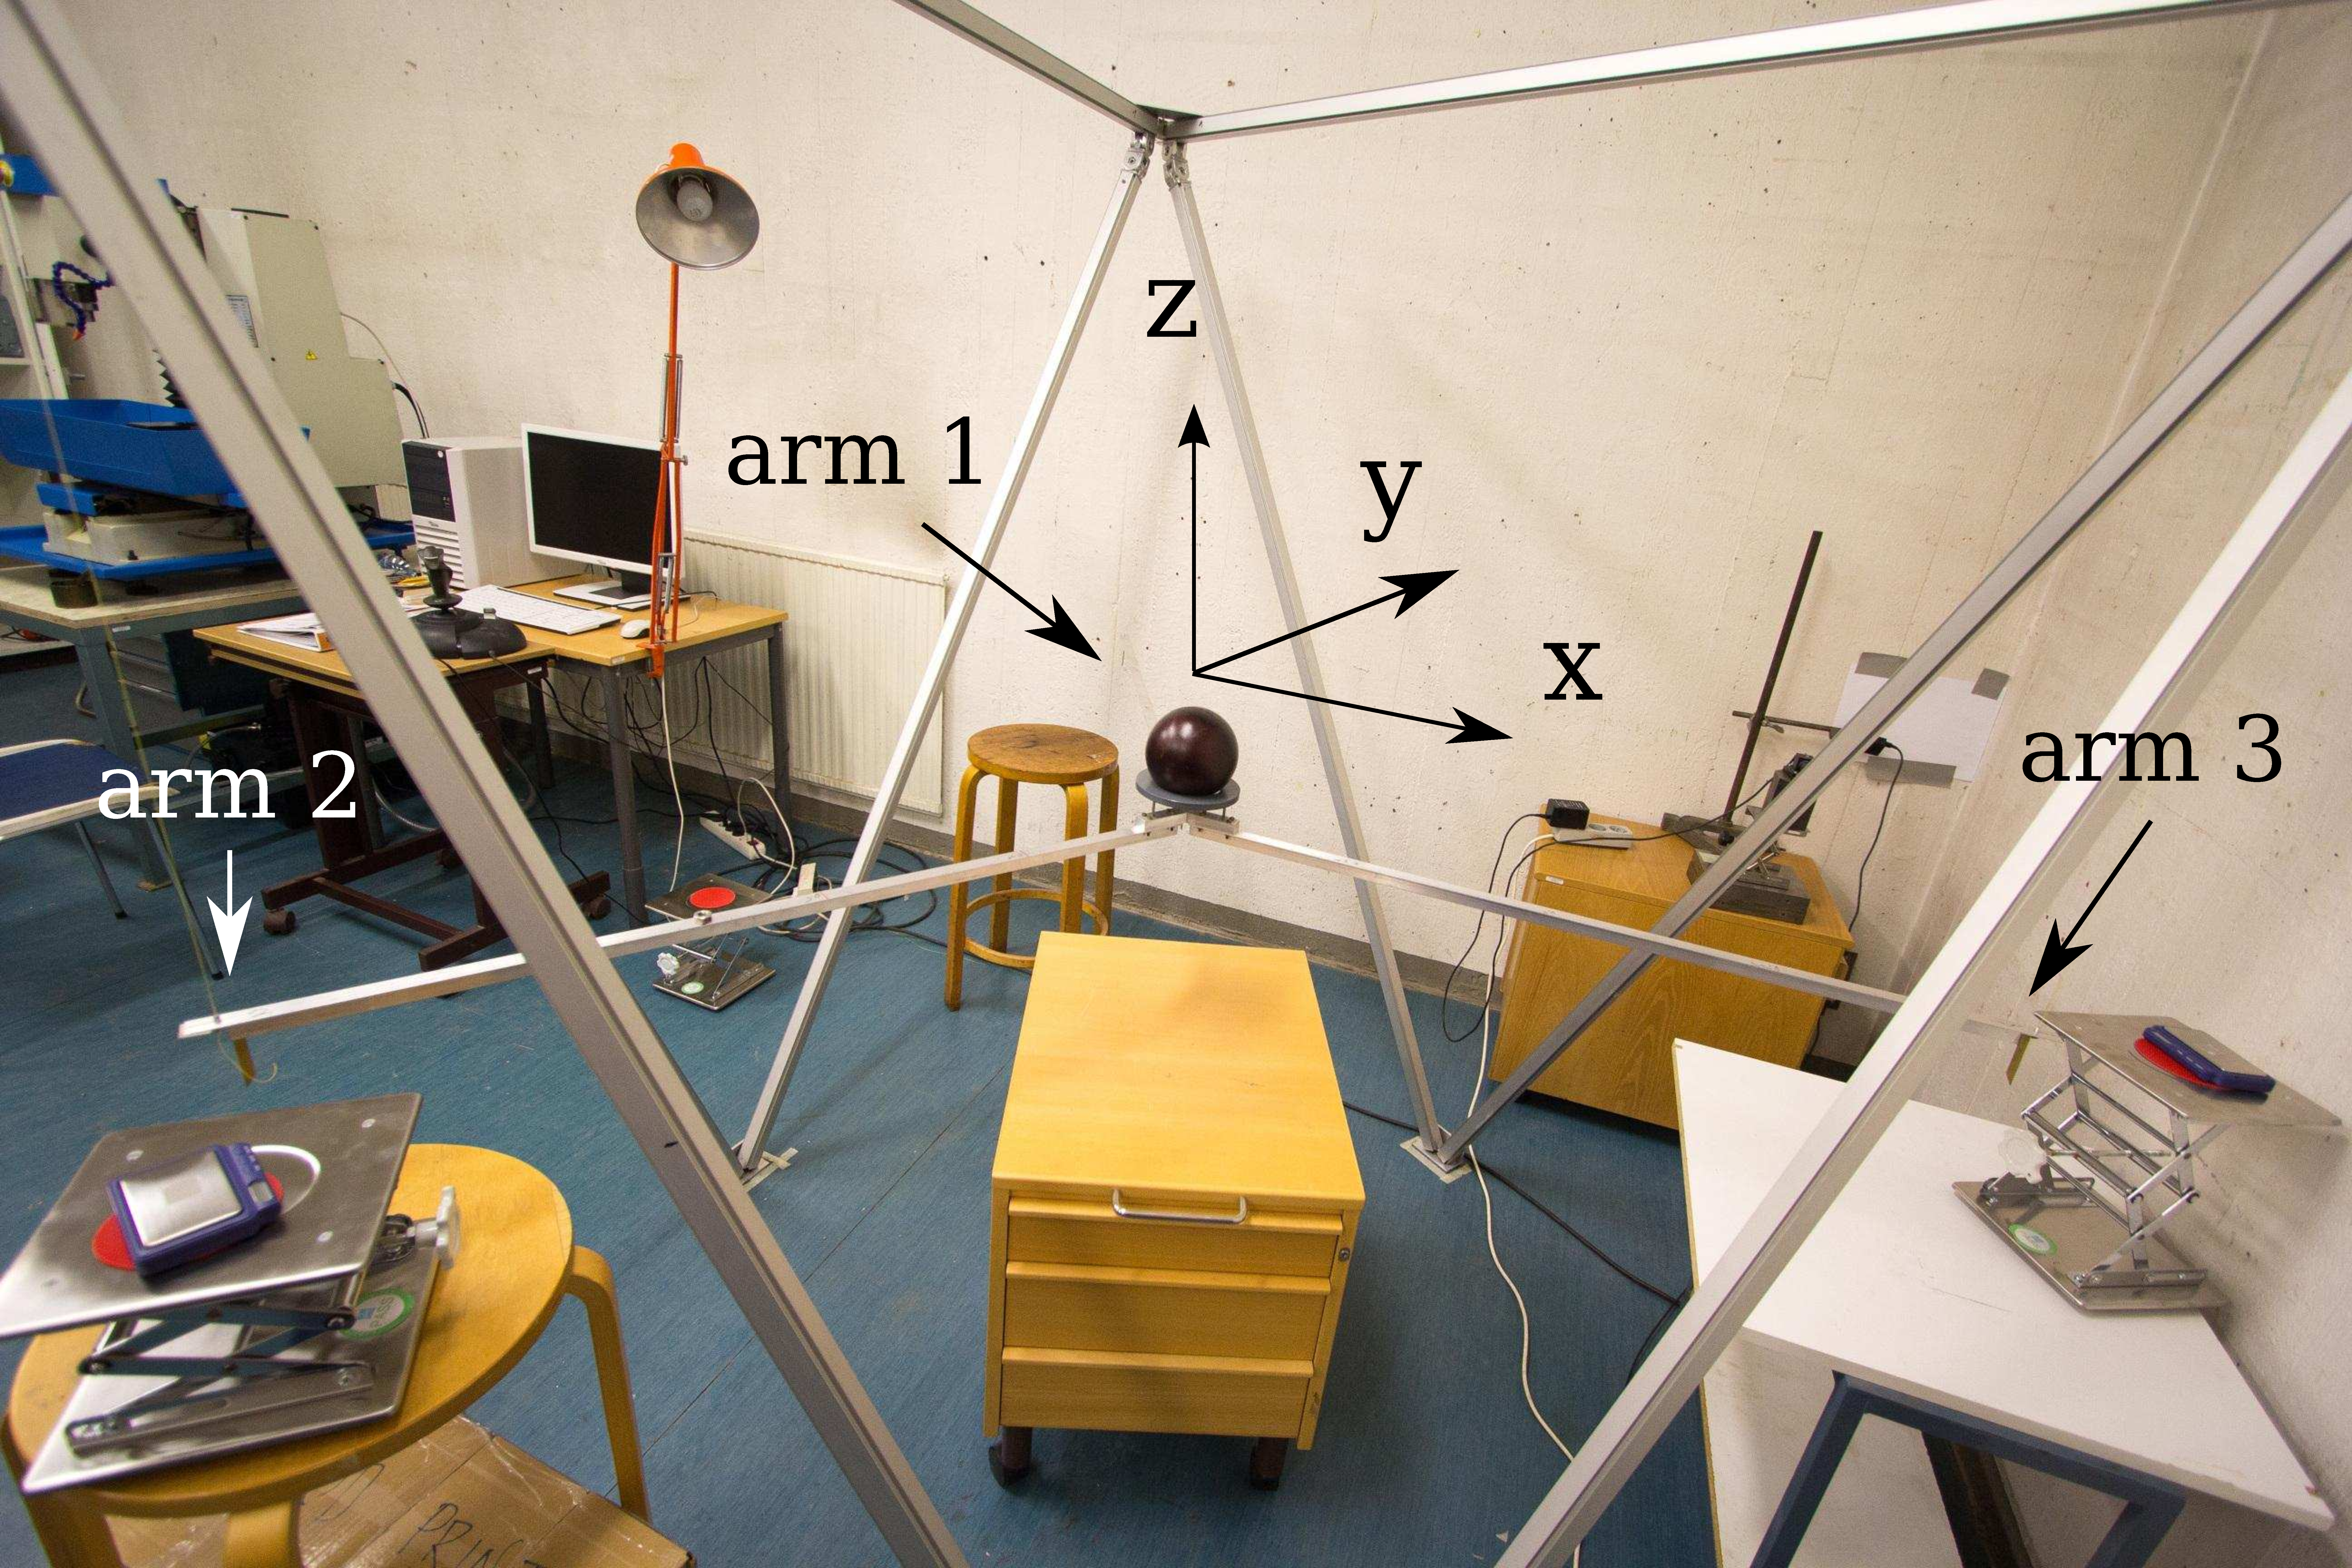
\includegraphics{PlatformCoordinates1}
	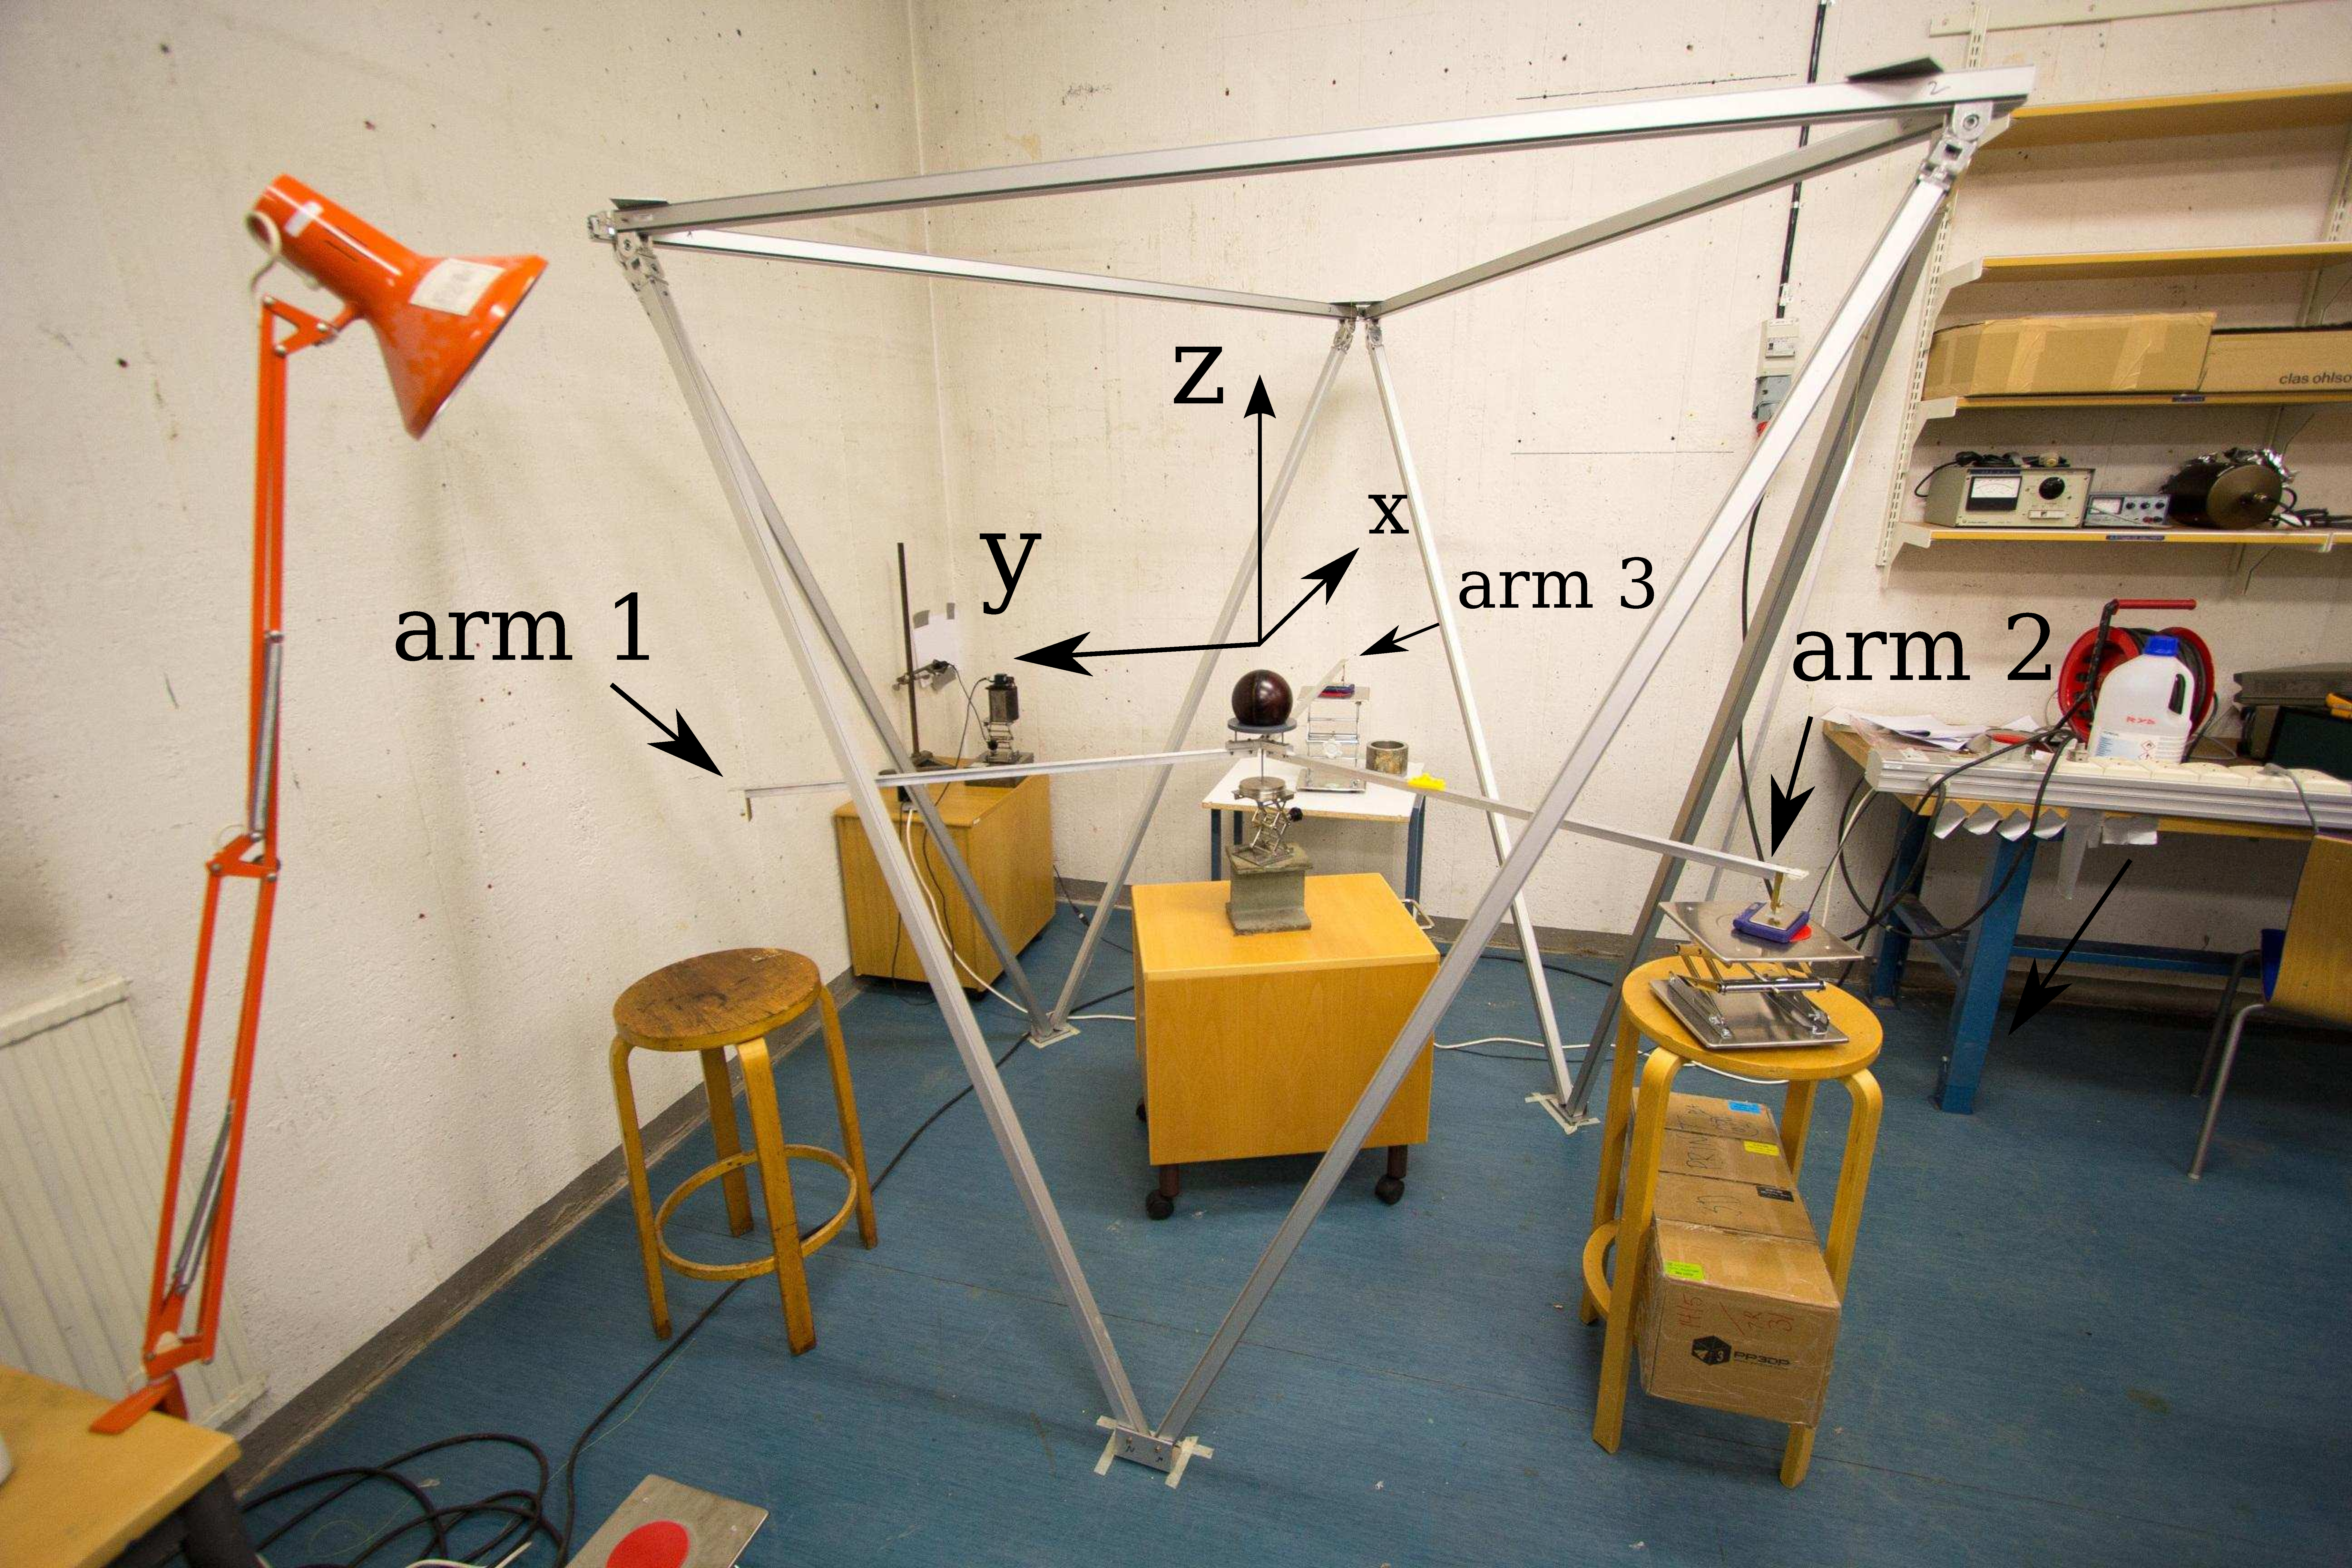
\includegraphics{PlatformCoordinates2}
	\caption{Two pictures showing the trifilar pendulum with the \emph{MUSCAT FFU} mounted on the plastic ring, also giving the coordinate system used for the measurements. The first picture shows the free pendulum, whereas the second shows the pendulum on the support points. The vector corresponding to $L$ is parallel to the $z$ axis, whereas the vectors for $R$ lie in the $xy$ plane. They look different on the picture due to perspective distortions.}
	\label{fig:Platform}
\end{figure*}

\section{Center of Gravity}

In a system of particles the \emph{center of gravity} can be given by the relation \cite{book:goldstein}
\begin{align}
	\vec{R} & = \frac{1}{M} \sum_{i} m_i \vec{r}_i \\
	\label{eq:SystemCoG}
	M & = \sum_{i} m_i
\end{align}

We can use this relation, since we treat the platform and the unit as single particles, i.~e. we have
\begin{align}
	\vec{R} & = \frac{m_{\textup{p}} \vec{r}_{\textup{p}} + m_{\textup{u}} \vec{r}_{\textup{u}}}{m_{\textup{p}} + m_{\textup{u}}} \label{eq:CogFull}
\end{align}

However, we do not know any of the coordinates $\vec{r}_i$. 
But since we are only interested in the position of the center of gravity of the unit, we can perform two measurements of the platform, with and without the unit, to extract the wanted information.

The measurement works by placing the platform on \emph{three} support points, given by sharp spikes.
The central spike is in the geometric center of the platform, and hence has the coordinate $\vec{s}_{\textup{c}} = (0, 0)$.
The other support points are attached to the end of each arm and placed on a precision scale. When placed on the spikes, the platform stands on three support points, which are the central spike and two arms, while one arm is always free in the air (figure \ref{fig:Support}).

\begin{figure}[b]
	\centering

	\begin{subfigure}{0.32\linewidth}
		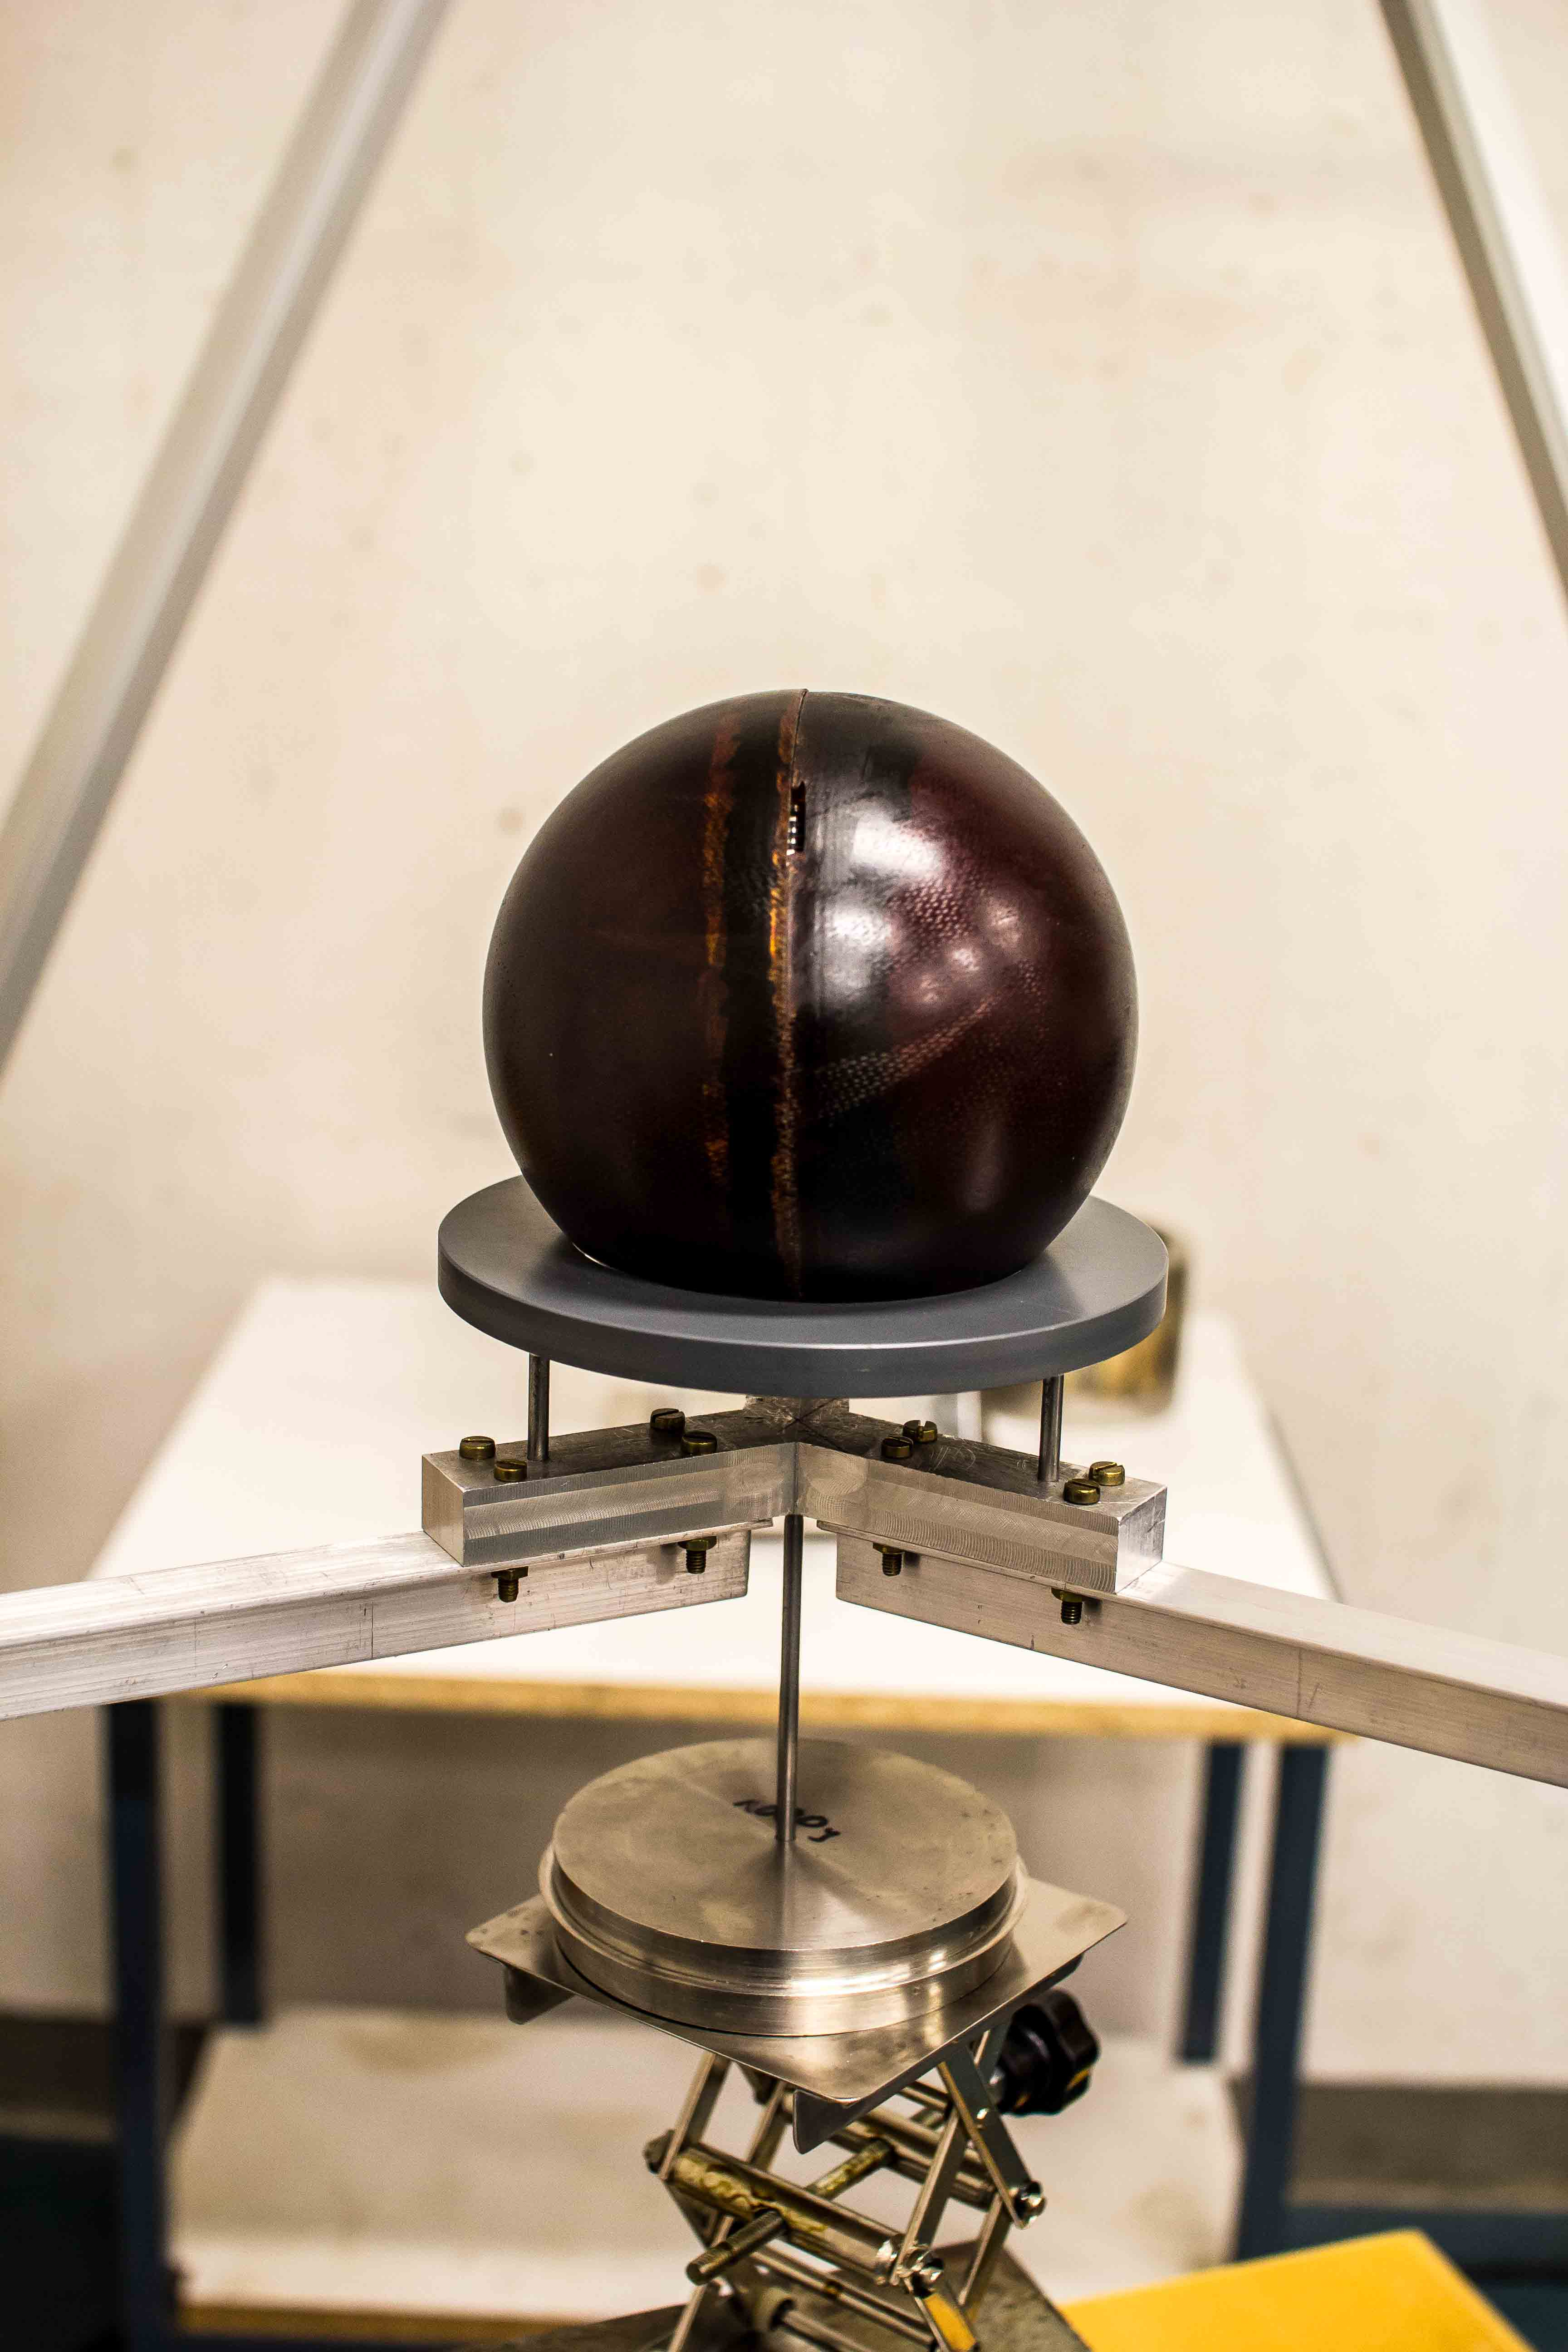
\includegraphics{Support1}
		\subcaption{}
	\end{subfigure}
	\begin{subfigure}{0.32\linewidth}
		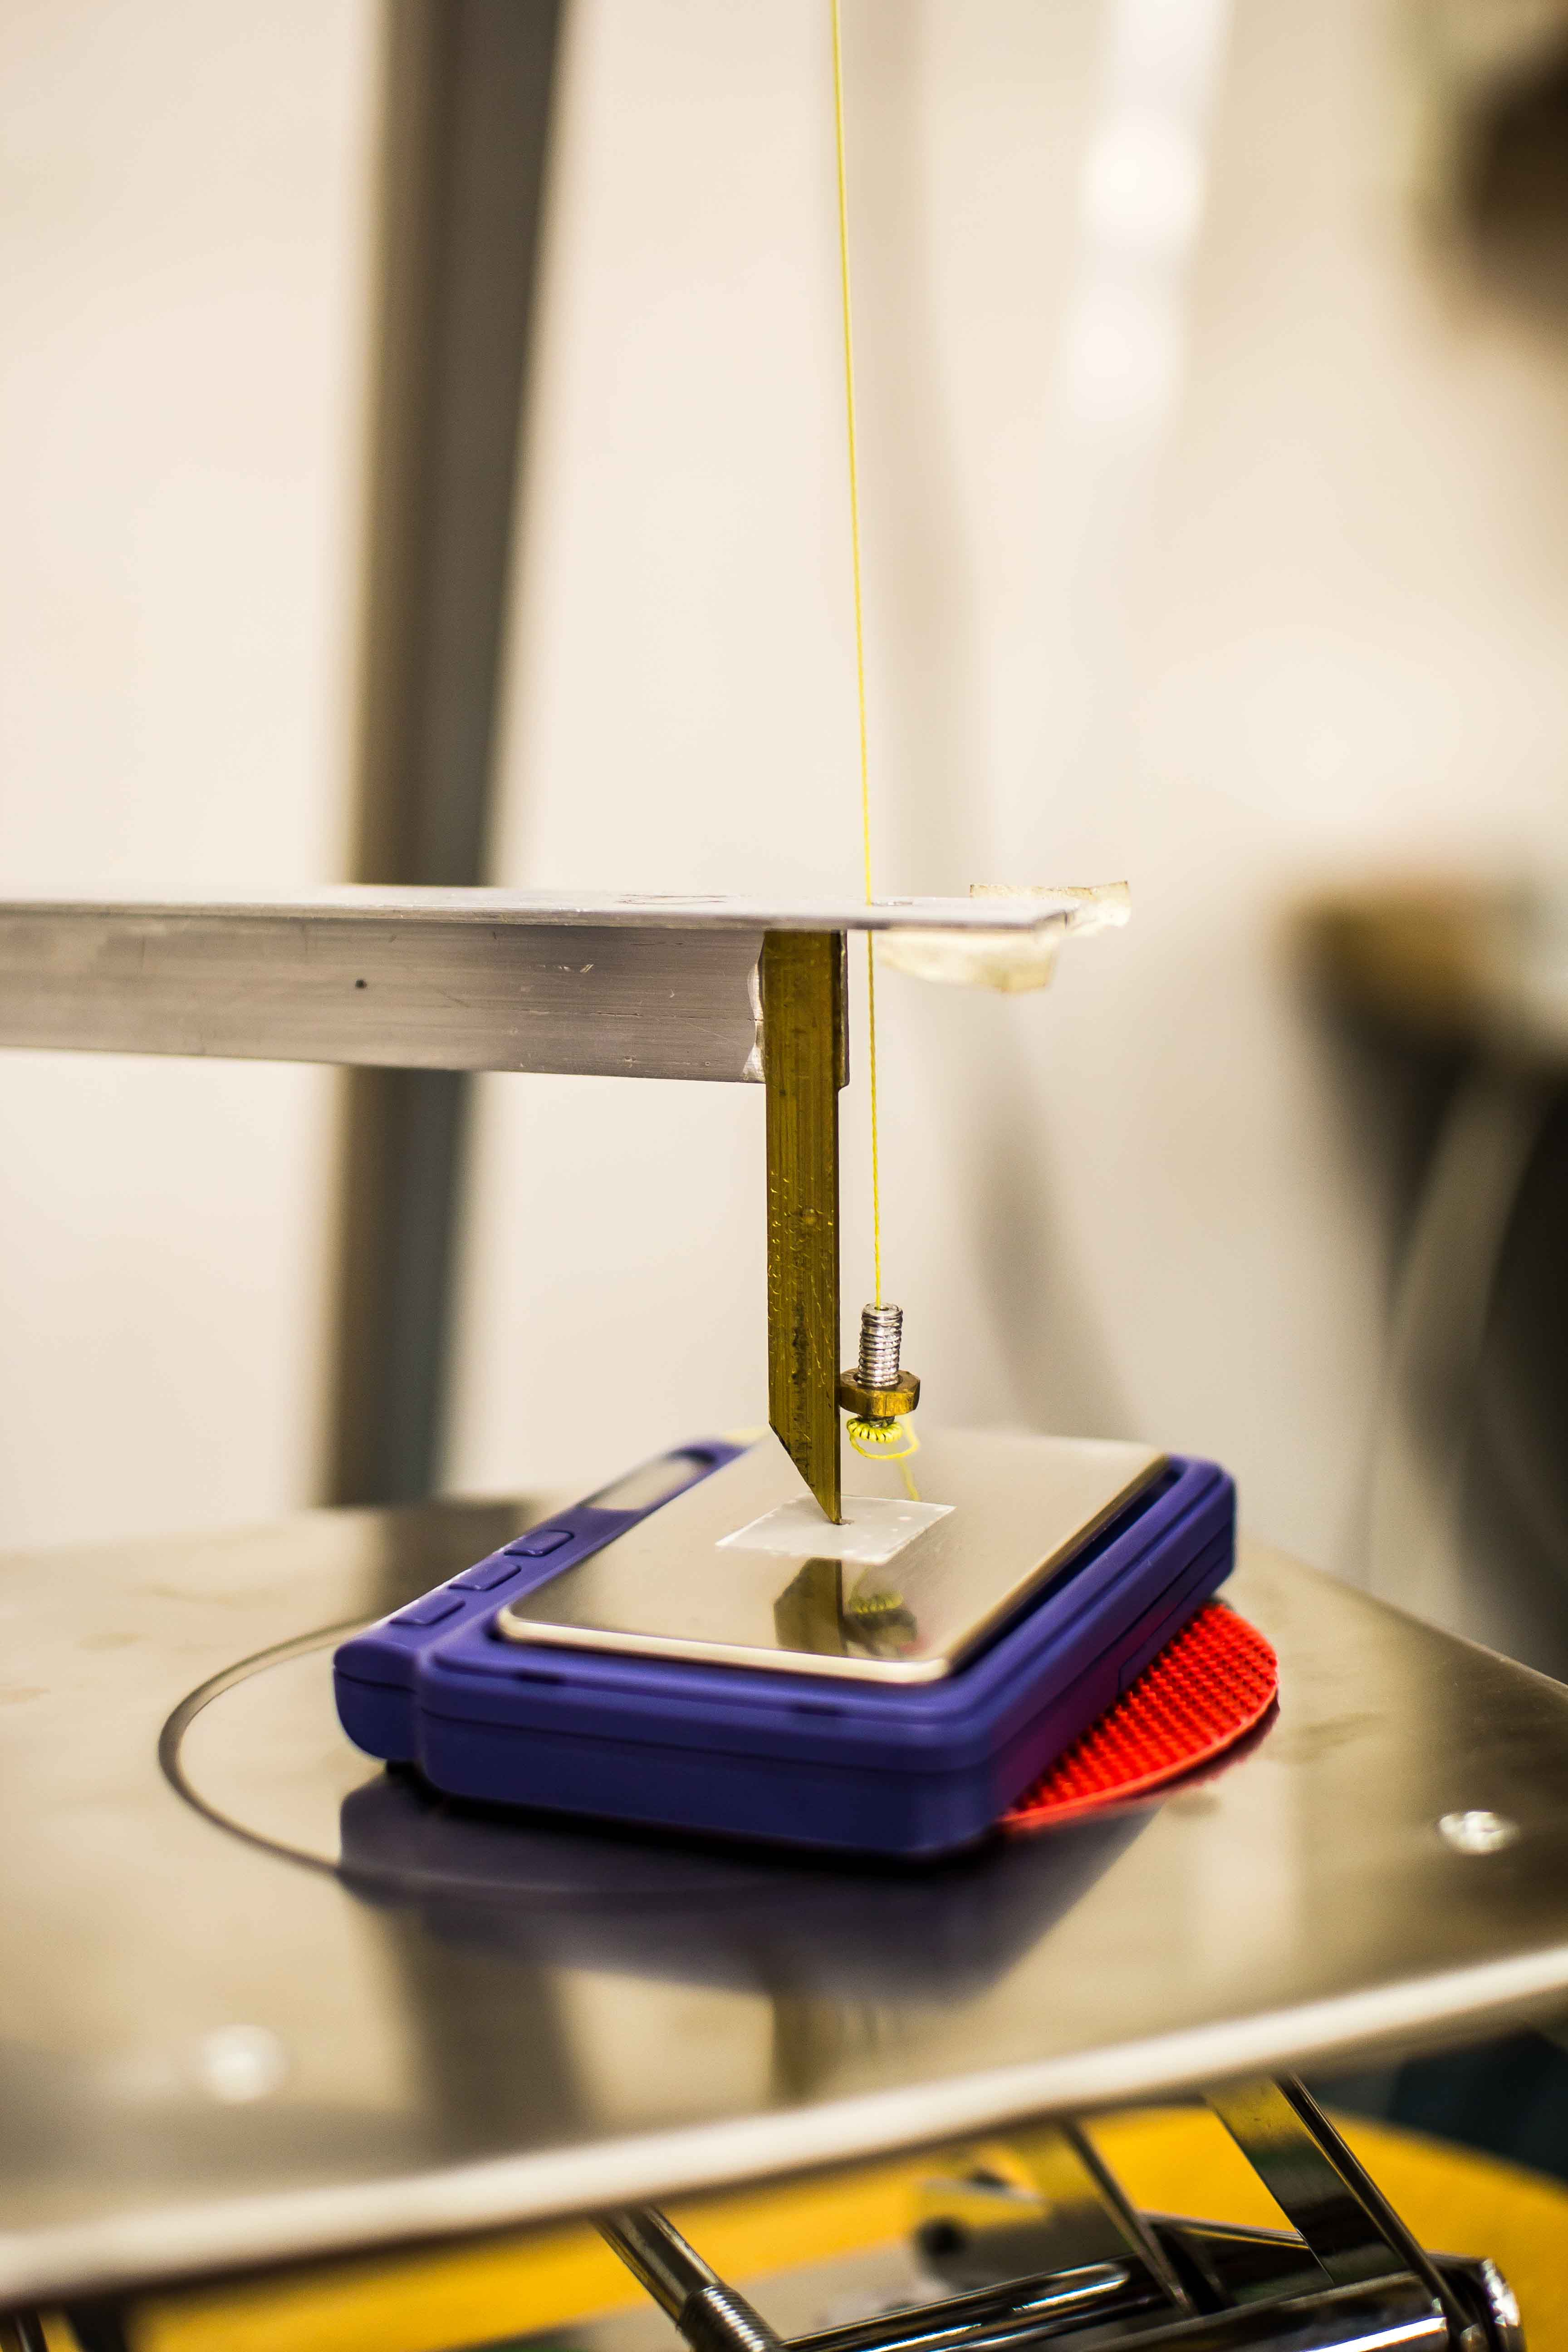
\includegraphics{Support2}
		\subcaption{}
	\end{subfigure}
	\begin{subfigure}{0.32\linewidth}
		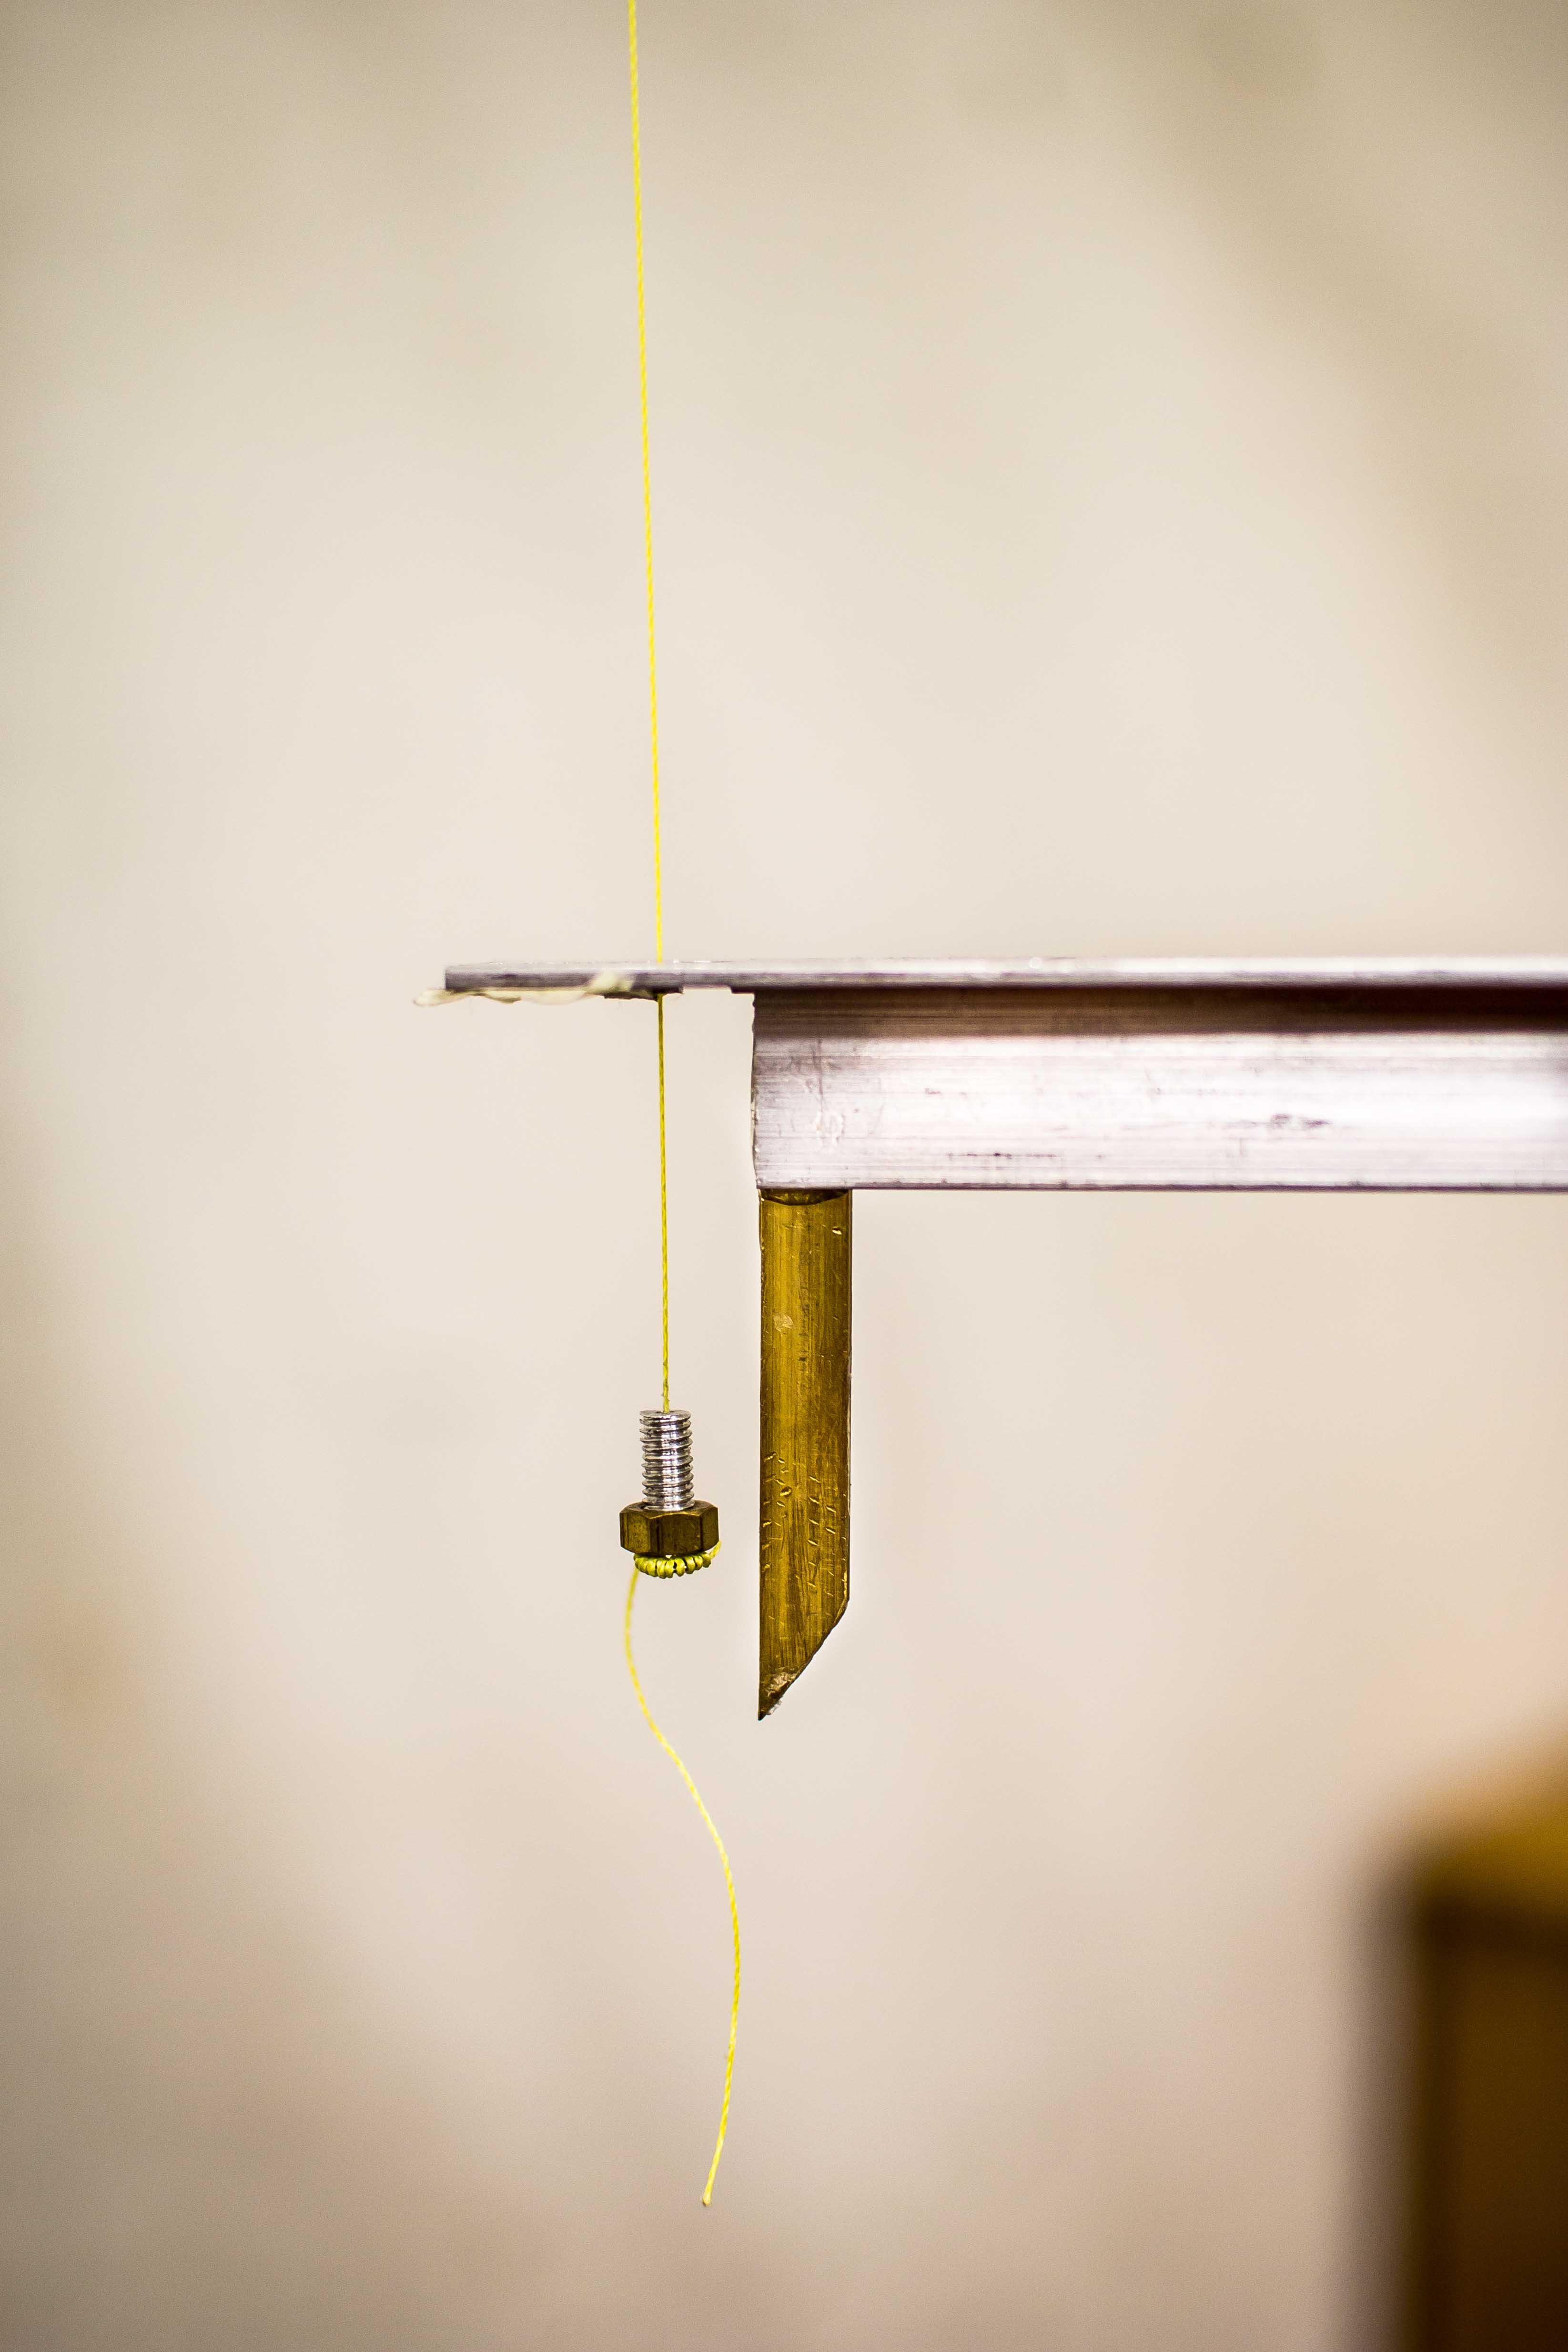
\includegraphics{Support3}
		\subcaption{}
	\end{subfigure}

	\caption{Fixed platform with \emph{MUSCAT FFU} on the central spike (a), support point on a scale (b) and the free arm (c).}
	\label{fig:Support}
\end{figure}

As the scales give the equivalent of a mass placed at the support point and the mass on all support points together sum up to $M$, we can write
\begin{align}
	\vec{R} & = \frac{(M - g_1 - g_2) \vec{s}_{\textup{c}} + g_1 \vec{s}_1 + g_2 \vec{s}_2}{M} \\
	& = \frac{g_1 \vec{s}_1 + g_2 \vec{s}_2}{M} & \comment{$\vec{s}_{\textup{c}} = (0,0)$}
\end{align}

where $g_i$ denote the mass equivalents measured by the scales.

Equating with \eqref{eq:CogFull} gives
\begin{align}
	m_{\textup{p}} \vec{r}_{\textup{p}} + m_{\textup{u}} \vec{r}_{\textup{u}} = g_1 \vec{s}_1 + g_2 \vec{s}_2
\end{align}

Repeating the measurement without the unit then gives
\begin{align}
	m_{\textup{p}} \vec{r}_{\textup{p}} = g_1' \vec{s}_1 + g_2' \vec{s}_2
\end{align}

And substracting the two equations hence yields the \emph{2D CoG} formula
\begin{align}
	\vec{r}_{\textup{u}} & =  \frac{(g_1 - g_1') \vec{s}_1 + (g_2 - g_2') \vec{s}_2}{m_{\textup{u}}}
	\label{eq:2DCoG}
\end{align}

where $g$ is the \emph{total g} value and $g'$ is the \emph{platform g} value. Hence, the difference $g-g'$ then represents the bare \emph{unit g} value as wanted.
The test mass can then be used to repeat this measurement under different conditions.
This gives statistics about the real center of gravity of the unit and since the mass and position of the test mass is known, it adds a known contribution to the values of the scales.

\subsection{Testing the single scale measurement}
\label{sec:SingleScale}

To check, if the above procedure works as expected, we need to test it against a known property.
Therefore, we select one arm to be tested and perform measurements using a test mass placed at different positions on the arm, see figure \ref{fig:TestMass}.

\begin{figure}[b]
	\centering
	\setkeys{Gin}{width=0.8\linewidth}
	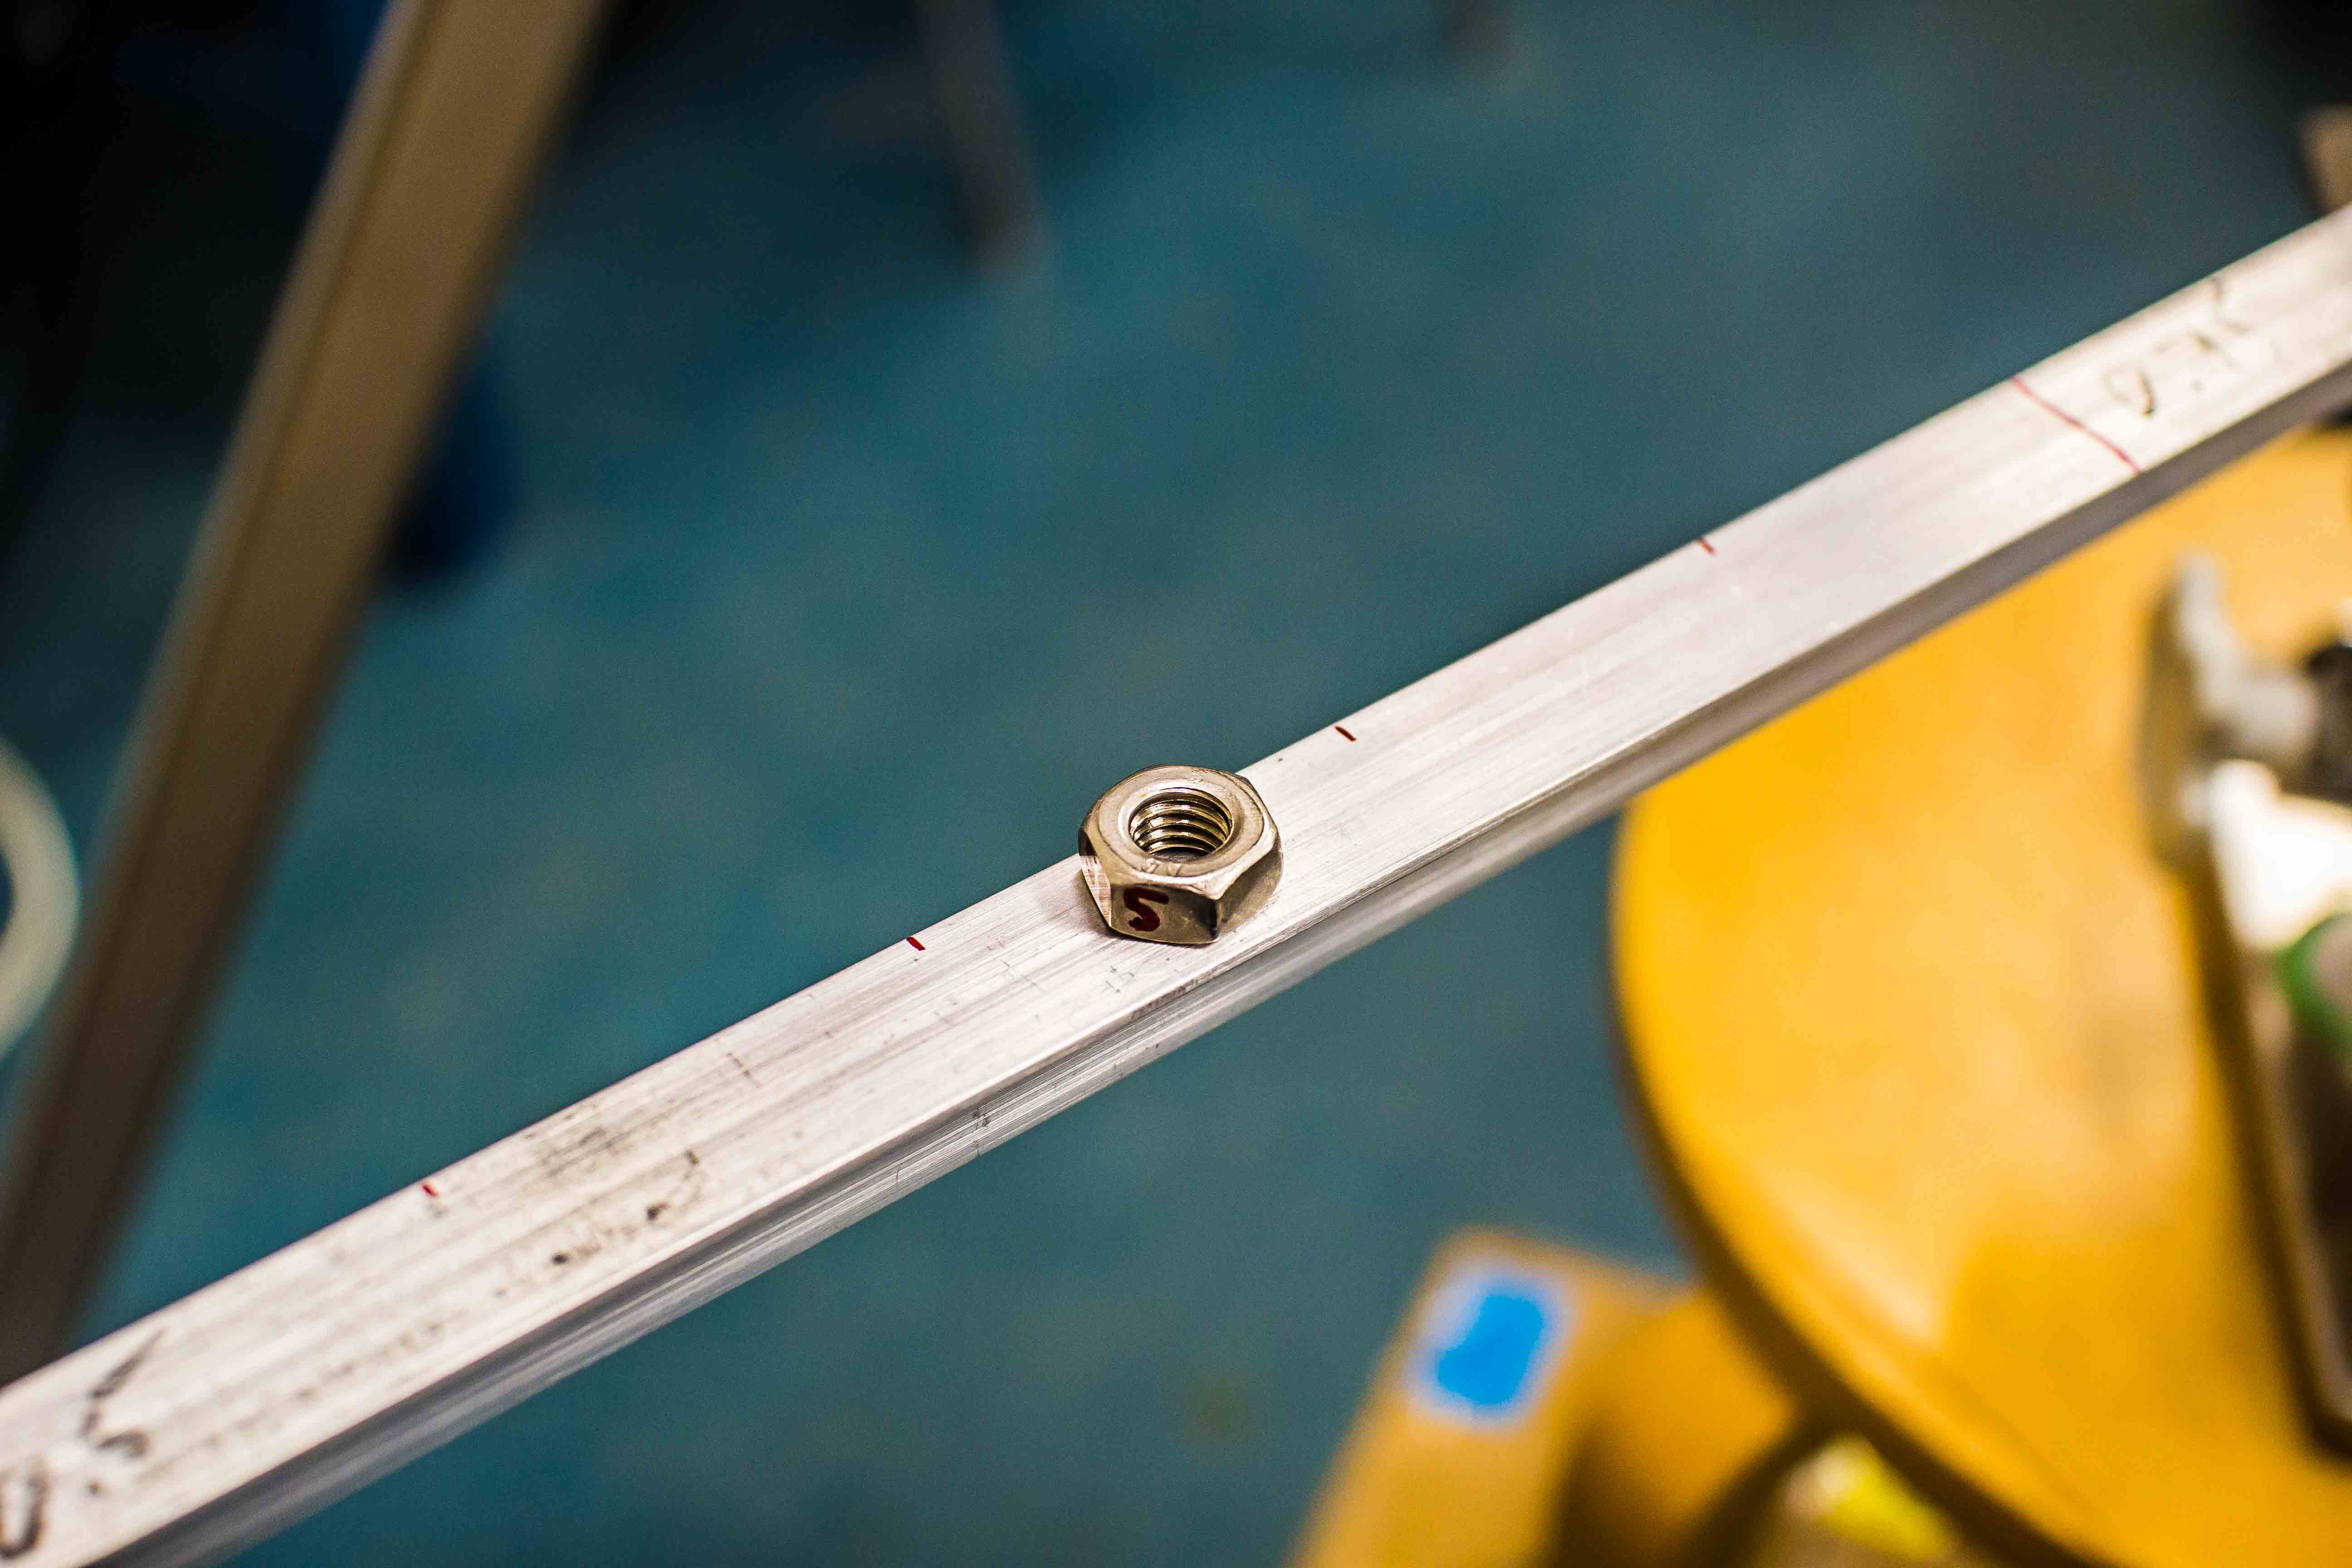
\includegraphics{TestMass}
	\caption{A nut as test mass placed on an arm.}
	\label{fig:TestMass}
\end{figure}

Assuming, that the test weight only affects the arm, which it is placed on, thus giving $g_2 = g_2'$, we find from \eqref{eq:2DCoG}
\begin{align}
	\vec{r} & = \frac{(g - g') \vec{s}}{m}
\end{align}

Taking the absolute value, we thus have
\begin{align}
	g & = \frac{m r}{s} + g'\\
	& = g_{\textup{t}}(r) + g'
	\label{eq:gt}
\end{align}

which predicts the result of the measurements to be a linear function in $r$ shifted by the constant value $g_1'$.

A test has then been performed on each arm with a nut of mass $10.40 \unit{g}$ placed at positions $r \in [25, 75]$~cm in steps of 5~cm, thus giving a total of 11 measurements.
To estimate the constant $g'$, we take the mean difference of these measurements between the obtained values of $g$ and $g_{\textup{t}}$.
This quantity is used again in many other plots and is thus given as
\begin{align}
	\delta g & \equiv \overline{g - g_{\textup{t}}}
	\label{eq:DeltaG}
\end{align}

where the bar denotes the mean over the measurements of the particular series.

Adding it to $g_{\textup{t}}$ places the theoretical curve directly upon the measured, thus making it easy to see any deviations.
As the platform was not in perfect equilibrium during the measurement, the values on the scales were not constant. Thus, a constant uncertainty of 0.2 g has been assumed for all measurements using the scales.
The results are given in figure \ref{fig:SingleScale} show a very good agreement with the theoretical prediction.
This procedure of using a test mass to obtain a series of $g$ measurement is used again in the next section.

\begin{figure}
	\centering
	\setkeys{Gin}{width=0.9\linewidth}
	\includegraphics{SingleScale/g1}
	\includegraphics{SingleScale/g2}
	\includegraphics{SingleScale/g3}
	\caption{Measurement curve of the single scale test. Each point represents one measurement of $g_i$ with an uncertainty of 0.2 g. The theoretical prediction $g_{\textup{t}}$ is shifted by the mean difference $\delta g$, such that the lines are placed upon each other. Only little to no deviation from the prediction can be observed. [\texttt{SingleScale.py}]}
	\label{fig:SingleScale}
\end{figure}

\subsection{2D center of gravity in a plane}
\label{sec:2DCoG}

The procedure of the section above was the extended to measure the center of gravity of a unit in the two-dimensional $xy$ plane of the platform.
Using the estimate of $g'$ from the previous section, we could measure the value $g$ with the unit and then find $g-g'$.
However, it was found, that it is very difficult to set up the platform exactly in the same way, such that the measured value $g'$ remains constant.
Thus, to determine the center of gravity, we take two series of $g$ on each arm, with and without the unit.
Substracting the two resulting curves for one arm then directly gives us a series of measurements of $g_i-g_i'$, of which the mean value can be taken as the final result.

To test the precision of this procedure, three weights have been placed on the platform.
Their weights and positions are given in table \ref{tab:3Mass}. The position given in cm refers to the distance of the weight to the center of the platform.
Since all positions and masses are known, the resulting center of gravity can be directly calculated by using equation \eqref{eq:SystemCoG}. The result is given as $\vec{R}_{\textup{t}}$ in table \ref{tab:3MassResults}.
Five positions of the test mass ranging from 25--75 cm in steps of 10 cm have been used to determine $g-g'$.
As a constant quality control, the curve $g_{\textup{t}} + \delta g$ is given as a reference for each curve of $g_i$ and $g_i'$. They are shown in figure \ref{fig:3MassGTest}.
The measured quantities are given in table \ref{tab:3MassValues}. The given uncertainties denote the standard deviation of the measured values.
Comparing the measured center of gravity with the one we have calculated, we note however, that measured point is displaced by roughly 3 mm on each axis, giving a total distance of 5 mm  to the predicted center of gravity. This is seen in table \ref{tab:3MassResults}, where $\vec{R}_m$ is for the measured center of gravity.
This can be due to systematic errors in the measurement procedure and has to be investigated further, if more precision is required. A detailed error calculation might be helpful to find out, if this error is due to lack of precision in the determination of the $g$ values.

\begin{table}
	\centering
	\begin{tabular}{r | r r r}
		\# & mass [g] & arm & position [cm] \\
		\hline
		1	&	10.40	&	1	&	25	\\
		2	&	48.07	&	2	&	50	\\
		3	&	10.54	&	3	&	50	\\
	\end{tabular}
	\caption{Properties and positions of the objects used for the 2D center of gravity determination test.}
	\label{tab:3Mass}
\end{table}

\begin{table}
	\centering
	\begin{tabular}{r | r r}
		& value & rel. $\sigma$ \\
		\hline
		$g_2 - g_2'$	&	21.777(99) g & 0.45 \% \\
		$g_3 - g_3'$	&	2.678(69) g & 2.56 \% \\
		$R_x$	&	$-119.0(1.6)$ mm & 1.32 \% \\
		$R_y$	&	$-273.3(1.2)$ mm & 0.45 \% \\
	\end{tabular}
\caption{Results of the 2D center of gravity determination of 3 test objects. [\texttt{CoG.py}]}
	\label{tab:3MassValues}
\end{table}

\begin{table}[t]
	\centering
	\begin{tabular}{r | r r}
		& x [mm] & y [mm] \\
		\hline
		$\vec{R}_{\textup{t}}$	&	$-116.6$	& $-269.0$ \\
		$\vec{R}_{\textup{m}}$	&	$-119.0$	& $-273.3$ \\
		$\vec{R}_{\textup{t}} - \vec{R}_{\textup{m}}$			&	2.4		& 4.3	\\
		$\frac{\Delta \vec{R}}{\vec{R}}$ &	2.0	\%	& 1.6 \% \\
	\end{tabular}
	\caption{Experimental results of the 2D center of gravity determination compared to the theoretical prediction using eq. \eqref{eq:SystemCoG}.}
	\label{tab:3MassResults}
\end{table}

\begin{figure}
	\centering
	\setkeys{Gin}{width=0.49\linewidth}
	\includegraphics{CoG/g2}
	\includegraphics{CoG/g2p}
	\includegraphics{CoG/g3}
	\includegraphics{CoG/g3p}
	\caption{Measured $g$ curves for the 2D center of gravity test plotted against the prediction $g_{\textup{t}}$ for verification of the measurement procedure. [\texttt{CoG.py}]}
	\label{fig:3MassGTest}
\end{figure}

\section{3D center of gravity}

Since we want to obtain the center of gravity of our unit in three dimensions, we need to combine two measurements of the 2D center of gravity as described in section \ref{sec:2DCoG}.
For example, by placing the unit in its original orientation, where the $z$ axis points up (here called $z+$), a measurements in the $xy$ plane of the platform gives the $x$ and $y$ components of the 3D center of gravity. See also figure \ref{fig:AxesCoG}.
Then rotating the unit by 90 degrees, such that the $y$ axis points downward ($y-$), the same measurement yields the x and z coordinates of the 3D center of gravity
Alternatively, we can let the $x$ axis point downward ($x-$) to obtain the $z$ and $y$ component from the measurement.

\begin{figure}
	\centering
	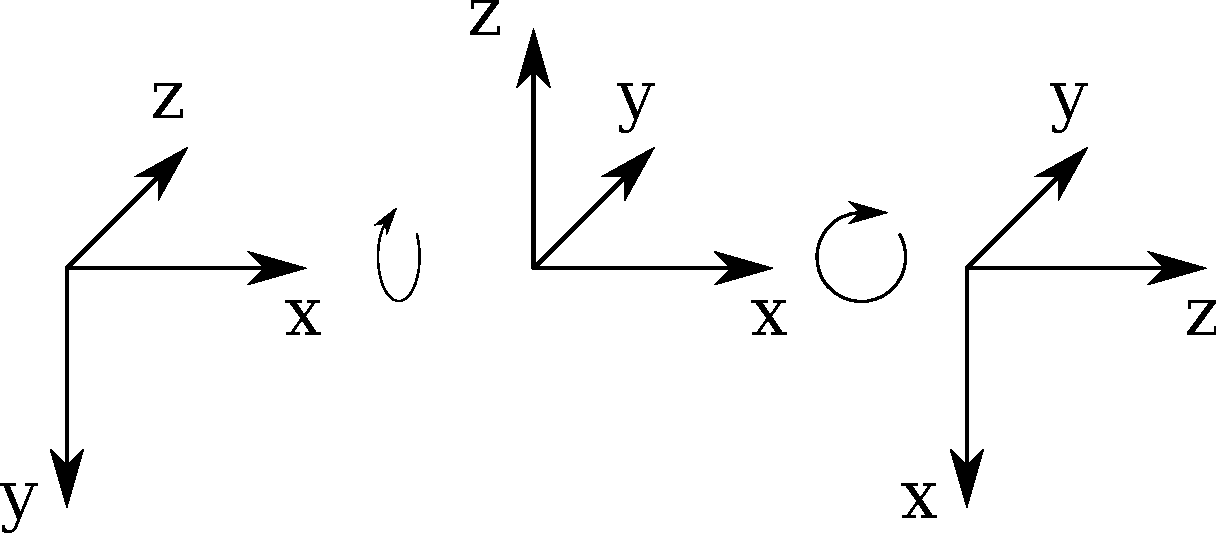
\includegraphics{AxesCoG}
	\caption{Possible orientations for center of gravity measurements. Starting with $z+$ in the middle, one obtains $y-$ and $x-$ by simple rotations.}
	\label{fig:AxesCoG}
\end{figure}

\section{Moment of inertia}

If we rotate the trifilar pendulum by a few degrees and let it move freely, the period of the resulting oscillation is directly related to the moment of inertia. Thus, to determine the moment of inertia, we need to measure that period of oscillation.
By analyzing the equations of motions of the trifilar pendulum, the relation connecting the two quantities can be simplified to \cite{report:ernest}
\begin{align}
	I = \frac{R^2}{(2\pi)^2 L} m g T^2
	\label{eq:I}
\end{align}

where $T$ denotes the period of the oscillation of the trifilar pendulum. $L$ is the length of the cables, that hold the platform and $R$ is the distance from the attachment point of these cables to the center of the platform. Figures \ref{fig:Platform} shows the two quantities on the real platform. The cables are parallel to the $z$ axis, however due to perspective distortions, they appear different in the picture.

The equation requires, that the center of gravity is in the geometric center of the platform.
For the generic case, the factor $\frac{R^2}{(2\pi)^2 L}$ has to be replaced by a more complicated expression.
However, since the no major deviations from the prediction have been observed, it is assumed, that this approximation suits the precision required in this experiment.

To measure the oscillation period, a fixed laser beam points on a tiny mirror, which is mounted on arm 3 of the platform.
The reflected beam is then projected onto a white paper on the wall behind the laser pointer and there filmed with a camera. 
When the pendulum rotates, the angle of the reflected beam changes, thus resulting in a periodic movement of the laser dot on the white paper.
A \emph{GoPro Hero} video camera is used to record a video of the laser dot at 240 frames per second.
To greatly enhance the contrast of the resulting video file, the room lighting must be turned off during measurement and the desk lamp at the platform used instead to work with the platform.
The camera mount and the laser dot is shown in figure \ref{fig:LaserDot}.

\begin{figure}
	\centering

	\begin{subfigure}{0.49\linewidth}
		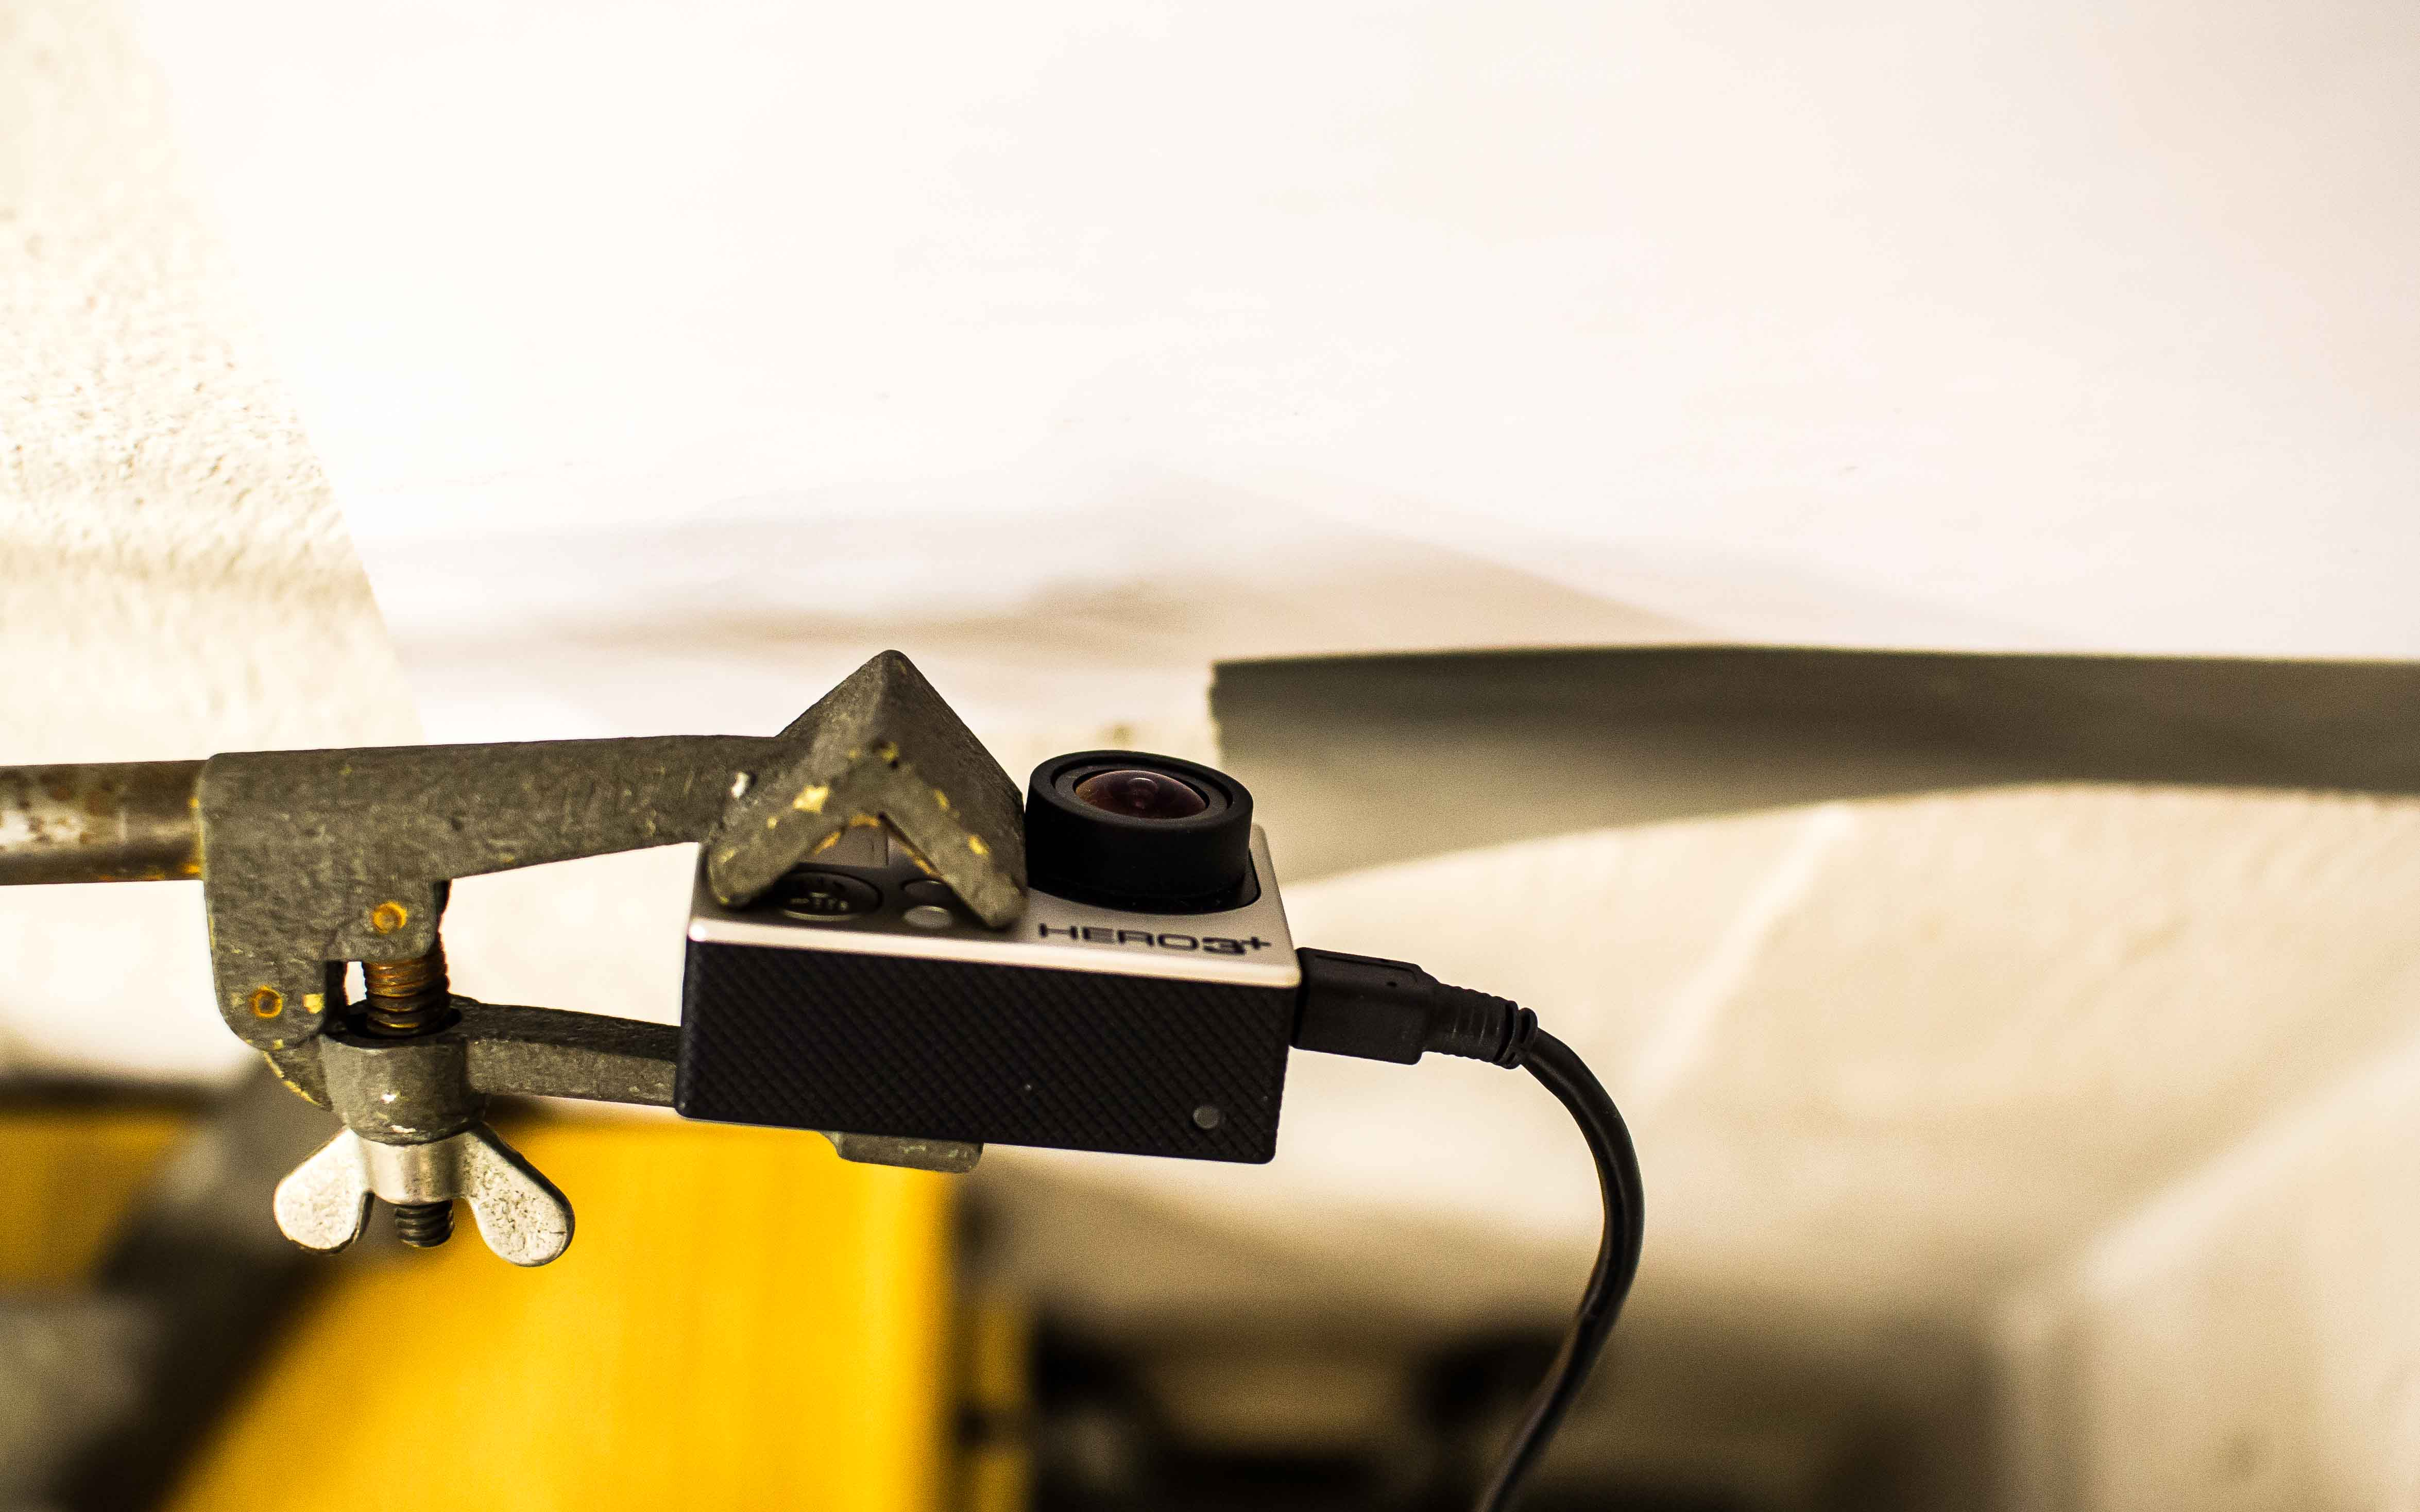
\includegraphics{Camera}
		\subcaption{}
	\end{subfigure}
	\begin{subfigure}{0.49\linewidth}
		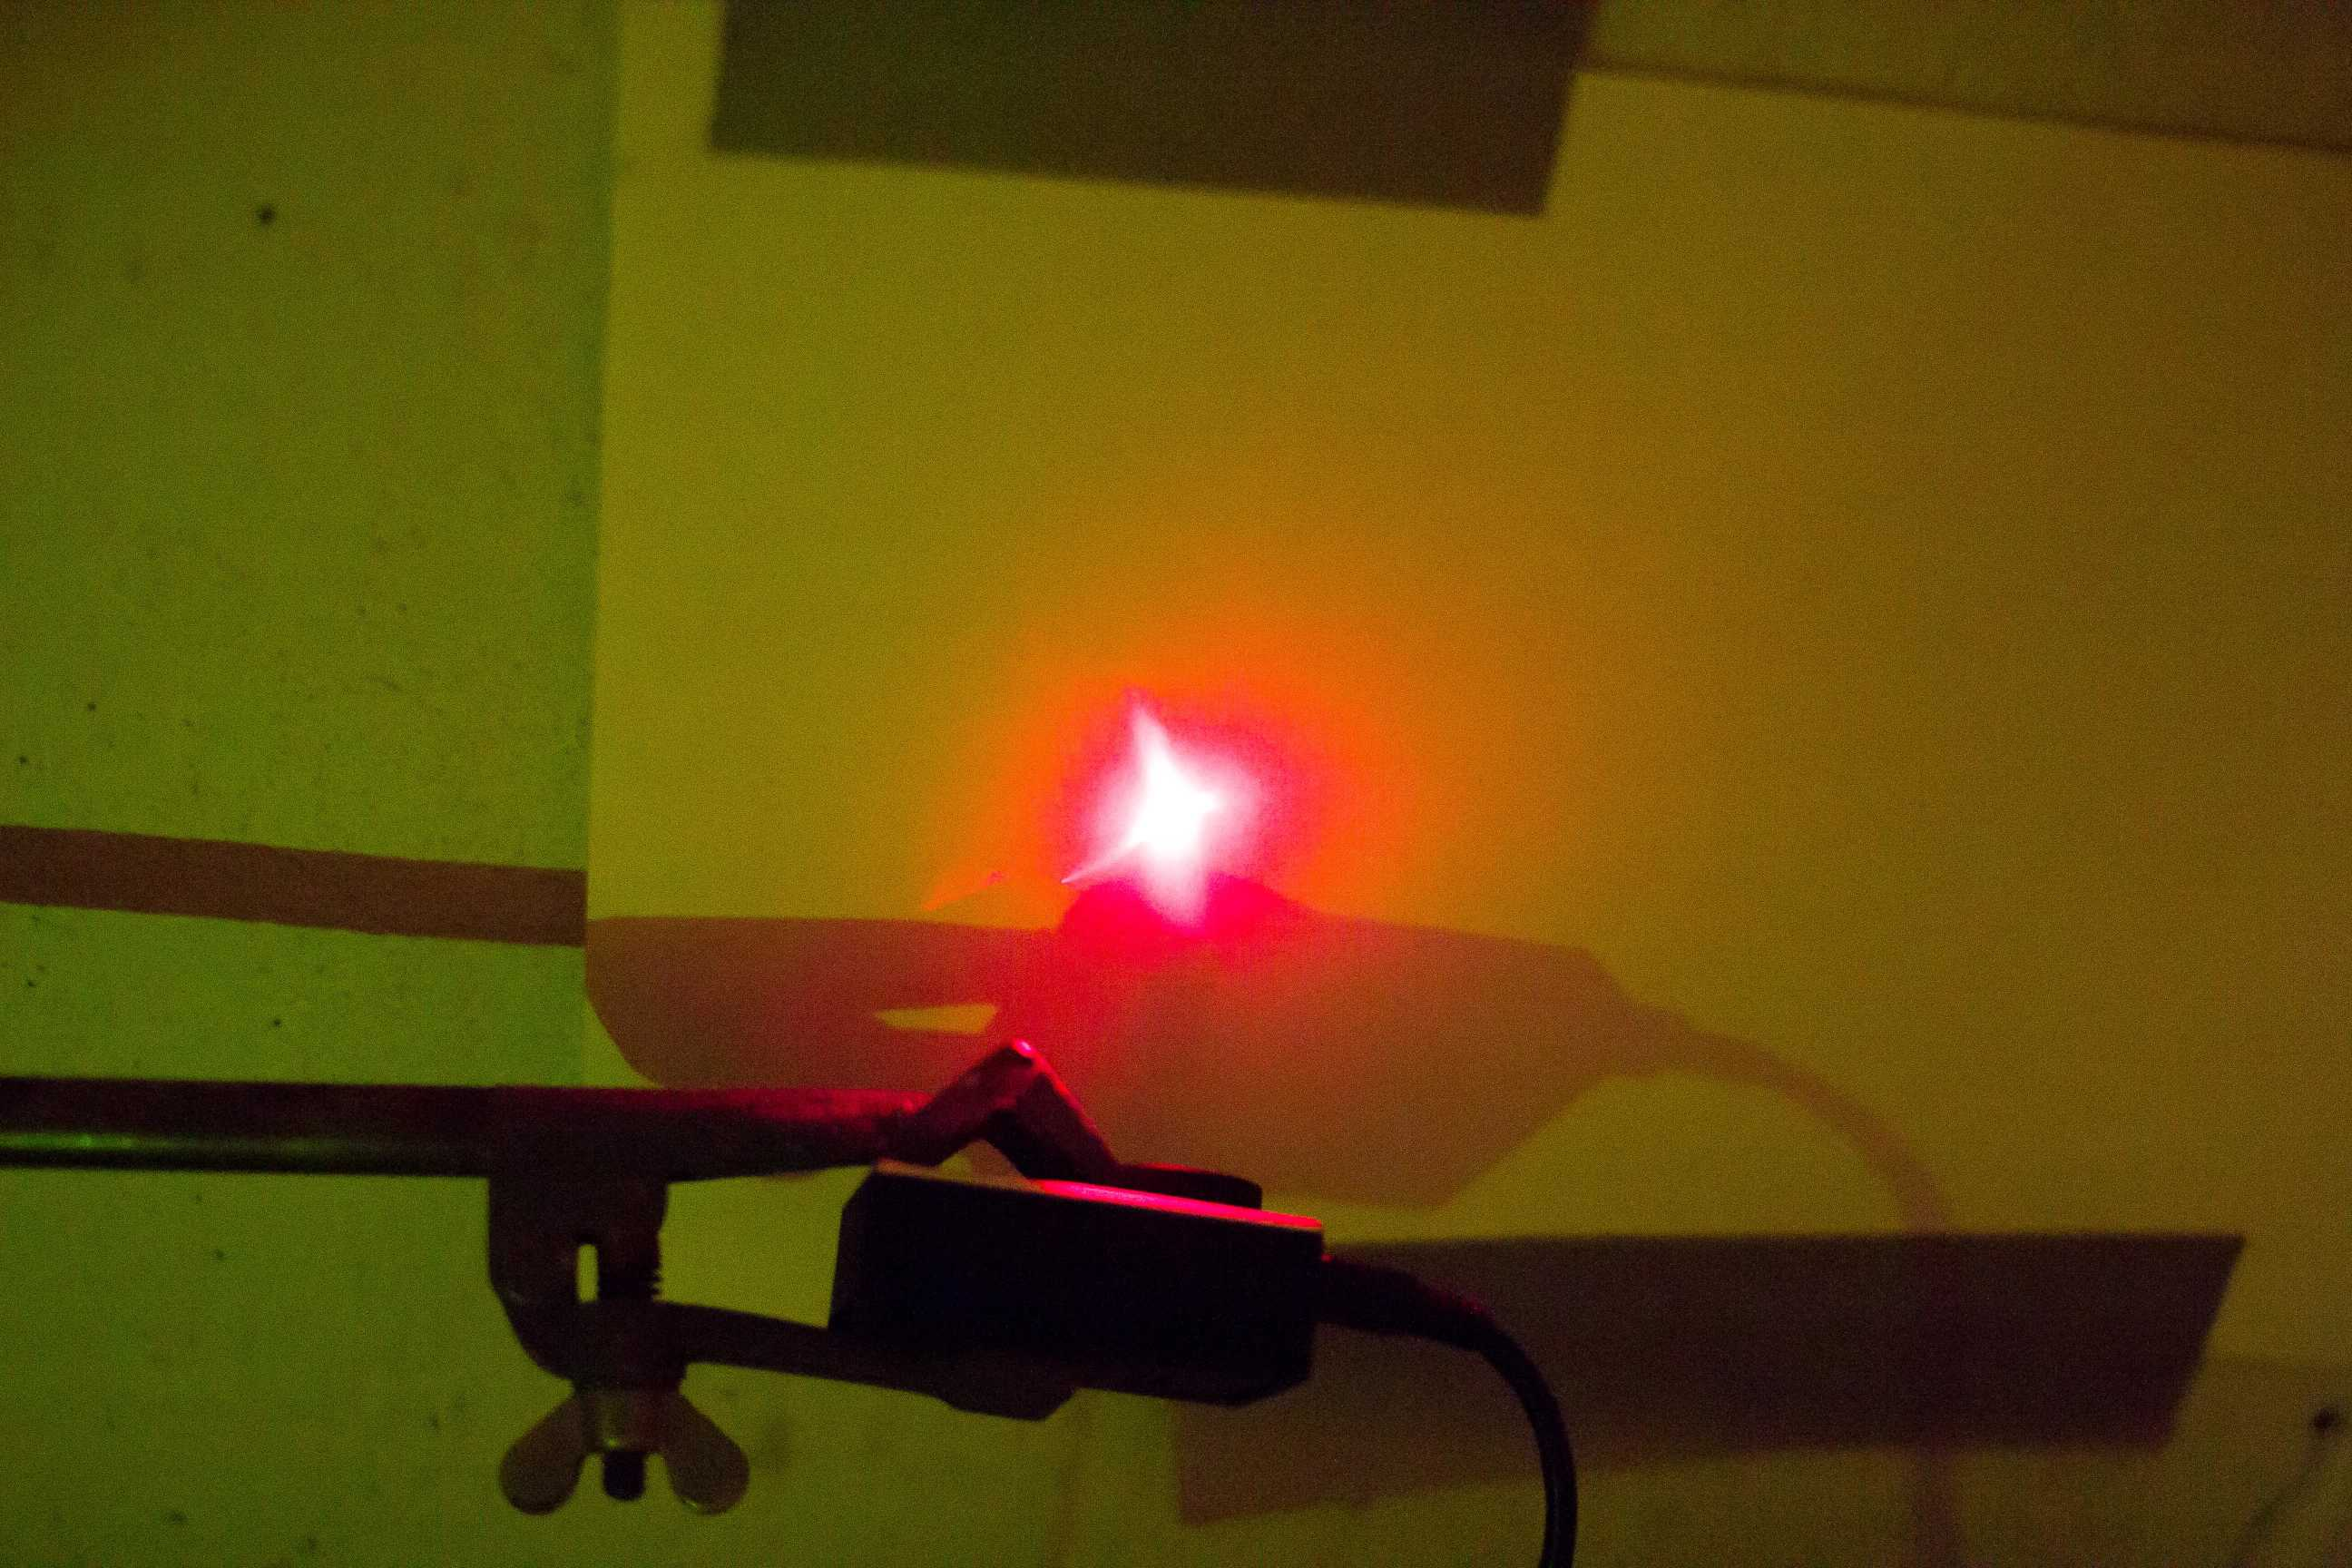
\includegraphics[clip=true,trim=0 0 0 33px]{LaserDot}
		\subcaption{}
	\end{subfigure}

	\caption{Mounted \emph{GoPro} camera (a) and projected laser dot with room lighting switched off (b).}
	\label{fig:LaserDot}
\end{figure}

To analyze a video, each frame is converted to \emph{HSV} (Hue-Saturation-Value) color space and filtered for the range (150,0,100) -- (349,255,255).
This selects only the pixels of the laser dot, as demonstrated in figure \ref{fig:VideoThreshhold}.
The first order moments of the filtered image for the $x$, resp. $y$ axis divided by the total area of the dot then give the coordinates of the point in a particular frame.

\begin{figure}
	\centering
	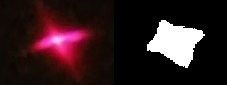
\includegraphics[width=0.7\linewidth]{video_threshhold}
	\caption{Image from a video capture of the \emph{GoPro} camera. The left side shows the original image and the right side shows the image filtered by the HSV range (150,0,100) -- (349,255,255). [\texttt{track.cpp}]}
	\label{fig:VideoThreshhold}
\end{figure}

The analysis is done by a simple program in \emph{C++}, which uses the \emph{OpenCV} (Open Source Computer Vision) library for image analysis.
Since this requires some computing power, analyzing a 20 s video with a resolution of \emph{848 x 480 / 240 fps} takes up to 30 s on an \emph{Intel i5-2540M}.

The platform rotation causes the laser dot to move roughly along a line on the wall. If the camera was mounted in perfect alignment with this line, there would be no movement in the $y$ direction of the recorded video file. As the camera is not aligned perfectly, the dot also slightly oscillates around the $y$ axis. However, this only scales the amplitude of oscillation in $x$ direction and does not change the actual perdiod. Hence, the $y$ component can be ignored.

Figure \ref{fig:PeriodFit} shows the spectrum of a recorded wave. As there are two peaks and we additionally assume a slight damping on longer measurements, a fit using two damped sine waves has been chosen.
The fitting function is thus defined as
\begin{align}
	f(\vec{A}, \vec{\tau}, \vec{T}, \vec{\delta}, C, t) & = \sum_{i=1}^2 A_i e^{-\tau_i t} \sin \left( \frac{2\pi}{T_i} t + \delta_i \right) + C
	\label{eq:FitFunction}
\end{align}

Of the two resulting waves, the one with the greater amplitude is taken as the wavefunction to determine $T$. The example curve along with the fit and the residual can be seen in figure \ref{fig:PeriodFit}.
The fit is performed as a least-square fit. Its success is heavily dependent on the initial parameters.
They have to be adjusted, if the period differs a lot between two measurements.

\begin{figure}
	\centering
	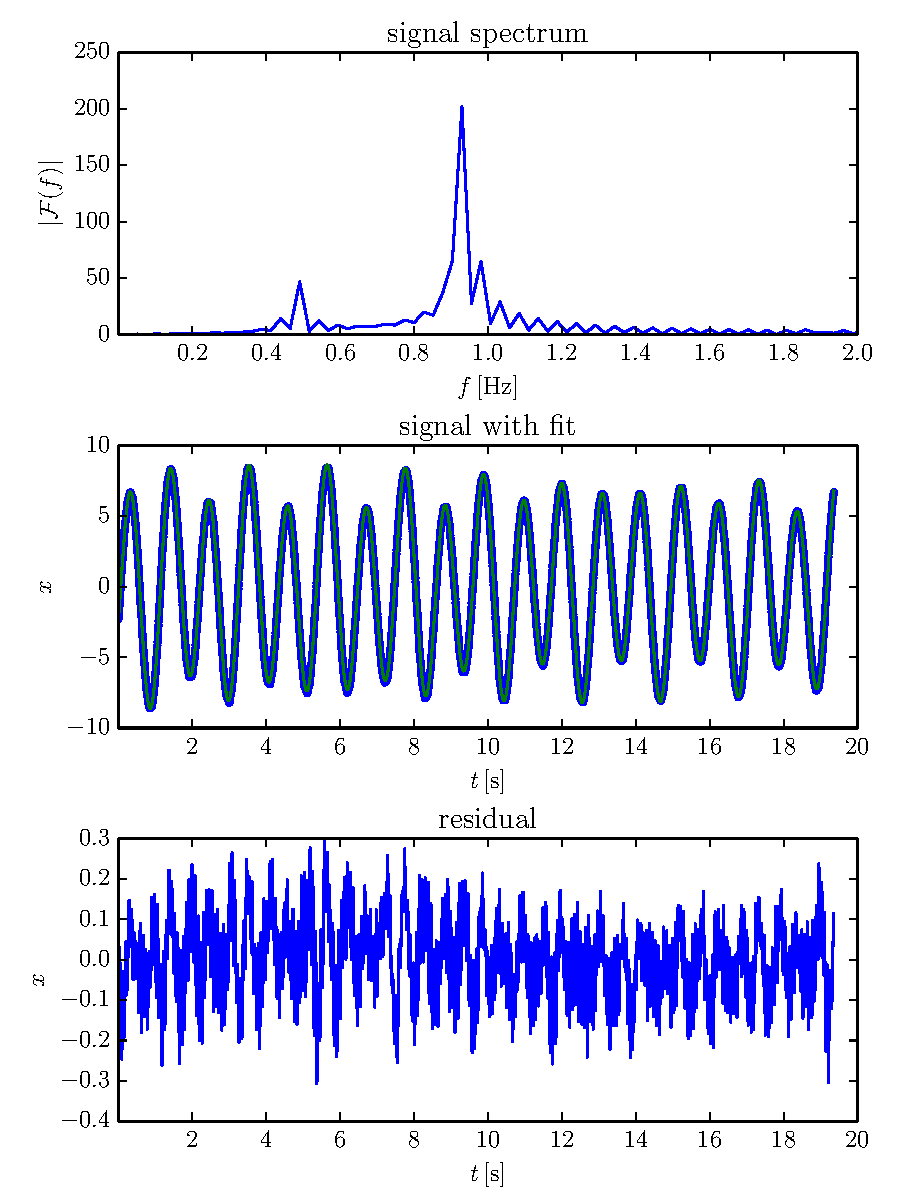
\includegraphics[width=\linewidth]{PeriodFit}
	\caption{Sample data from the $x$ component of a tracked video file showing the spectrum and the raw signal with the fit performed using function \eqref{eq:FitFunction}, as well as the difference between the fit and the data. The signal is shifted to the origin for better readability of the results. No unit on the vertical axes is given, since the overall magnitude is irrelevant for the frequency of oscillation. [\texttt{signal.py}]}
	\label{fig:PeriodFit}
\end{figure}

\subsection{Characterization}

To gather information about the precision of the measurement procedure and to find out, which recording duration of the video measurement is suitable, three series were taken with different recording durations.
One series consists of placing two nuts as a test mass with a total weight of 20.94 g on one arm at the positions from 25--75 cm in steps of 5 cm.
The chosen recording durations were 5, 10 and 20 s.

Again, we test the measurement against a theoretical prediction.
The theoretical moment of inertia of a single object of mass $m$ at distance $r$ is given by
\begin{align} 
	I_{\textup{t}} & = m r^2
	\label{eq:It}
\end{align}

So, as we move the test mass, the measured moment of inertia should rise as $r^2$.

The moment of inertia of multiple objects is just the sum of the individual moments. Thus, our measurement series is shifted by a constant value compared to the prediction $I_{\textup{t}}$. This constant then simply is the moment of the bare platform, which is finally evaluated in this measurement
Thus, by adding the mean difference between the measurement and the prediction to $I_{\textup{t}}$ places the two curves on each other, allowing easy verification of the prediction.
We denote this quantity with
\begin{align}
	\delta I & \equiv \overline{I - I_{\textup{t}}}
	\label{eq:DeltaI}
\end{align}

For the measurement uncertainty, we have an error in the quantities $R$, $L$, $m$ and $T$. The values of $R$ and $L$ are obtained with a tape measure and thus have the same error of $\Delta R = \Delta L = 0.5$ mm. The error in $m$ is $\Delta m = 0.5$ g. For $T$ the error is taken from the uncertainty of the least-square fit and is thus different for each measurement. For a 5 s video it is usually of order $10^{-5}$ s.
The error in $I$ is then given by

\begin{align}
	\Delta I & = \left| \frac{\partial I}{\partial R} \right| \cdot | \Delta R | + \left| \frac{\partial I}{\partial L} \right| \cdot | \Delta L | \\ &\;\;\;\; + \left| \frac{\partial I}{\partial m} \right| \cdot | \Delta m |  + \left| \frac{\partial I}{\partial T} \right| \cdot | \Delta T |\\
	& = \left( 2 \frac{\Delta R}{R} + \frac{\Delta L}{L} + \frac{\Delta m}{m} + 2 \frac{\Delta T}{T} \right) I
	\label{eq:IErr}
\end{align}

The resulting plots of the three measurement series are given in figure \ref{fig:Inertia}.
As can bee seen in the figures, the measured moments follow the prediction quite well. One can see a slight increase with the longer recording duration.
The numerical results for the platform moment are given in table \ref{tab:Inertia}, with the uncertainties given as standard deviations of each measurement series.
One can see, that the overall uncertainty of the measurement is in the already range of $\pm 0.00035 \unit{kg~m^2}$ for a 5 s measurement and reduces only slightly, as the measurement duration gets longer. For comparison, the two nuts, used as test mass, with a total weight of $20.94\,\unit{g}$ placed at $25\,\unit{cm}$ produce a moment of inertia of $I \approx 0.0013~\unit{kg\,m^2}$.
Therefore, for practical purposes, a measurement duration from 5--10 $\unit{s}$ can be recommended.

\begin{figure}[t]
	\centering
	\includegraphics{Inertia/5s}
	\includegraphics{Inertia/10s}
	\includegraphics{Inertia/20s}
	\caption{Measurement series for the inertia characterization with different recording durations plotted against the parabolic prediction $I_{\textup{t}}$ of eq. \eqref{eq:It}. The measurement curve is shifted by the average mean $\delta I$ to place the curves upon each other. [\texttt{Inertia.py}]}
	\label{fig:Inertia}
\end{figure}

\begin{table}
	\centering
	\begin{tabular}[h]{r | r  r}
		video duration [s] & $I_{\textup{p}}$ [$\unit{kg\,m^2}$] & rel. $\sigma$ \\
		\hline
		5	& 0.23479(35)	& 0.15 \% \\
		10	& 0.23452(29)	& 0.12 \% \\
		20	& 0.23448(21)	& 0.09 \% \\
	\end{tabular}
	\caption{Computed platform moment and errors derived from the calibration curves. [\texttt{Inertia.py}]}
	\label{tab:Inertia}
\end{table}

\section{Inertia Tensor}

The inertia tensor in matrix representation is given as
\begin{align}
	I = 
	\begin{pmatrix}
		I_{xx} & I_{xy} & I_{xz} \\
		I_{xy} & I_{yy} & I_{yz} \\
		I_{xz} & I_{yz} & I_{zz}
	\end{pmatrix}
\end{align}

where $I_{ij}$ are the \emph{moment of inertia coefficients}.
It thus takes 6 independent measurement to get the full inertia tensor.

Defining an arbitrary normalized vector
\begin{align}
	\vec{n} & = \alpha \vec{x} + \beta \vec{y} + \gamma \vec{z}
\end{align}

where $\alpha^2 + \beta^2 + \gamma^2 = 1$, we write the moment of inertia as \cite{book:goldstein}
\begin{align}
	I & = I_{xx} \alpha^2 + I_{yy} \beta^2 + I_{zz} \gamma^2 + 2 I_{xy} \alpha \beta + 2 I_{yz} \beta \gamma + 2 I_{zx} \gamma \alpha
\end{align}

Using this representation, we can find a simple set of measurements along an axis to deduct the whole inertia tensor.
By measuring the moment of inertia on a diagonal axis, i.~e. mounting the unit at an angle of $45^{\circ}$, we obtain simple expressions for elements.
Table \ref{tab:InertiaAxes} lists the six orientations and resulting expressions for the measured moments of inertia.

From now on, the notation given in the table is used, e.~g. orientation $xx$ means measuring along the x axis, whereas $xy$ means measuring along the diagonal axis given by $\vec{n} = \frac{\vec{x} + \vec{y}}{\sqrt{2}}$.
Thus, if we want to determine the element $I_{yz}$ and measure $I$ in the $yz$ axis, we first also need to obtain $I_{yy}$ and $I_{zz}$ and then find $I_{yz} = I - \frac{I_{yy} + I_{zz}}{2}$ from our previous measurement.

\begin{table}
	\centering
	\begin{tabular}{c | l l l}
		orientation	& definition	& $\vec{n}$	& I \\
		\hline
		xx & $\alpha = 1$							& $\vec{x}$								& $I_{xx}$ \\
		yy & $\beta = 1$							& $\vec{y}$								& $I_{yy}$ \\
		zz & $\gamma = 1$							& $\vec{z}$								& $I_{zz}$ \\
		xy & $\alpha = \beta = \frac{1}{\sqrt2}$	& $\frac{\vec{x} + \vec{y}}{\sqrt{2}}$	& $I_{xy} + \frac{I_{xx} + I_{yy}}{2}$ \\
		xz & $\alpha = \gamma = \frac{1}{\sqrt2}$	& $\frac{\vec{x} + \vec{z}}{\sqrt{2}}$	& $I_{xz} + \frac{I_{xx} + I_{zz}}{2}$ \\
		yz & $\beta = \gamma = \frac{1}{\sqrt2}$	& $\frac{\vec{y} + \vec{z}}{\sqrt{2}}$	& $I_{yz} + \frac{I_{yy} + I_{zz}}{2}$ \\
	\end{tabular}
	\caption{Orientations with unit vectors and resulting formulas for the moment of inertia measurement.}
	\label{tab:InertiaAxes}
\end{table}

\subsection{Parallel axis theorem}

By simply measuring the moments of inertia in the given orientations, we obtain the inertia tensor in the center frame of the unit.
However, the more interesting quantity is the inertia tensor of the unit in the center of mass frame.
The parallel axis theorem states that for a body with the center of gravity displaced by the perpendicular distance $R$, the measured moment if inertia is
\begin{align}
	I & = I_c + m R^2
\end{align}

where $I_c$ is the actual moment of inertia in the center of gravity frame of the body.
We thus have to subtract the term $m R^2$ from all our measurements, where $R$ is the distance from 3D center of gravity to the measuring axis.
The distance of a point $\vec{p}$ from a line $\vec{x} = \vec{a} + t \vec{n}$ can be calculated by
\begin{align}
	R & = || (\vec{a} - \vec{p}) - ( (\vec{a} - \vec{p}) \cdot \vec{n}) \vec{n} ||
\end{align}

And since the axes all have their origin in $\vec{a} = \vec{0}$, we simply have
\begin{align}
	R & = || \vec{p} - (\vec{p} \cdot \vec{n}) \vec{n} ||
\end{align}

\section{Analysis of the MUSCAT FFU}

To apply the whole procedure, the Free-Falling Unit (FFU) from the \emph{MUSCAT} project has been analyzed.
Since the unit has the shape of a sphere, it is easily possible to mount it in the required orientations. 

Unfortunately, the FFU did not fit well on the platform, as the three spikes in the middle had a too big distance from each other to support the unit.
Additionaly, the spherical shape make it difficult to rotate the unit by exactly 45 or 90 degrees.
To overcome this issue, a plastic ring was made, which fits onto the three spikes in the center of the platform and has a smaller inner radius, such that the unit fits well onto the ring.
In order to mount the unit in the desired angle, two small pins were attached to the ring. On the other side, three tiny holes with a diameter of a about 1 mm were drilled into the sphere. The two pins and the three holes allow us to mount the sphere in six different orientations on the platform, which correspond exactly to the six axes as given in table \ref{tab:InertiaAxes}.
Figure \ref{fig:PinsHoles} shows the plastic ring on the platform with the two pins and the three corresponding holes on the spherical FFU.
More details on the construction is given in appendix \ref{seq:ConstructAxes}.
Unfortunately, the axes names drawn currently on the unit surface have the $x$ and $y$ axes swapped compared to the coordinate system given here. This is corrected in all measurements shown here, but has to be taken into account for future measurements!

\begin{figure}
	\centering

	\begin{subfigure}{0.49\linewidth}
		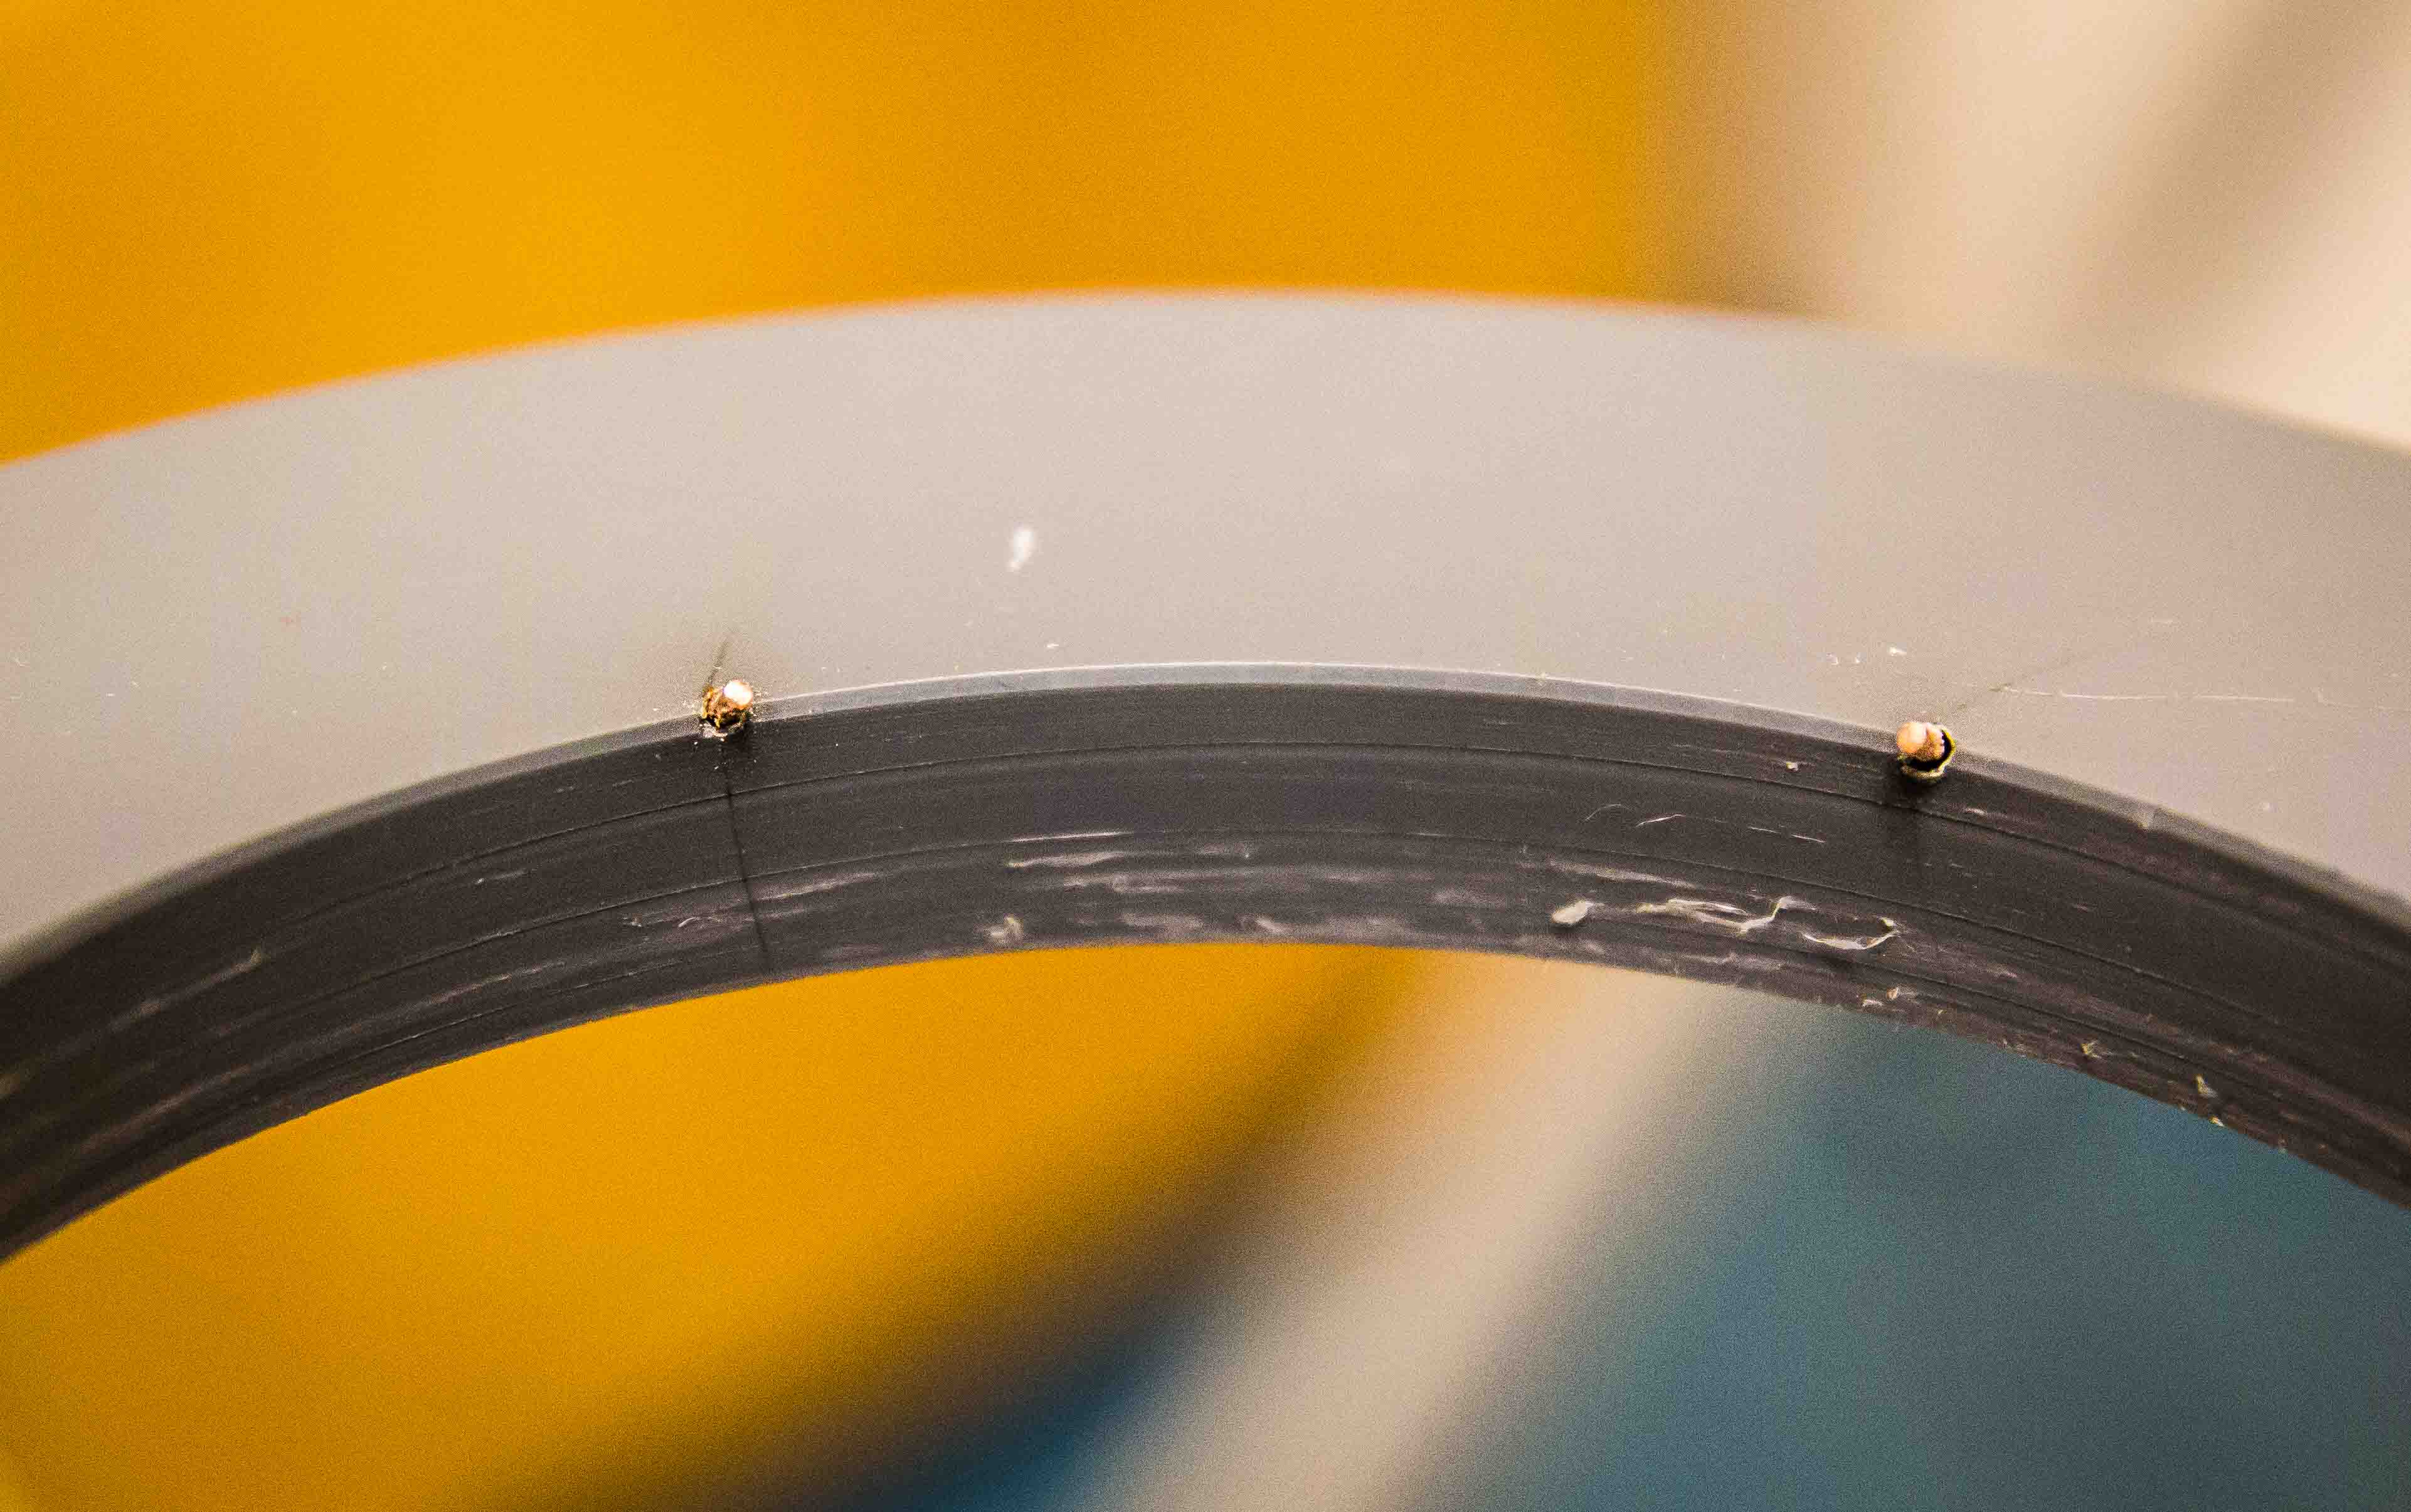
\includegraphics{Pins}
		\subcaption{}
	\end{subfigure}
	\begin{subfigure}{0.49\linewidth}
		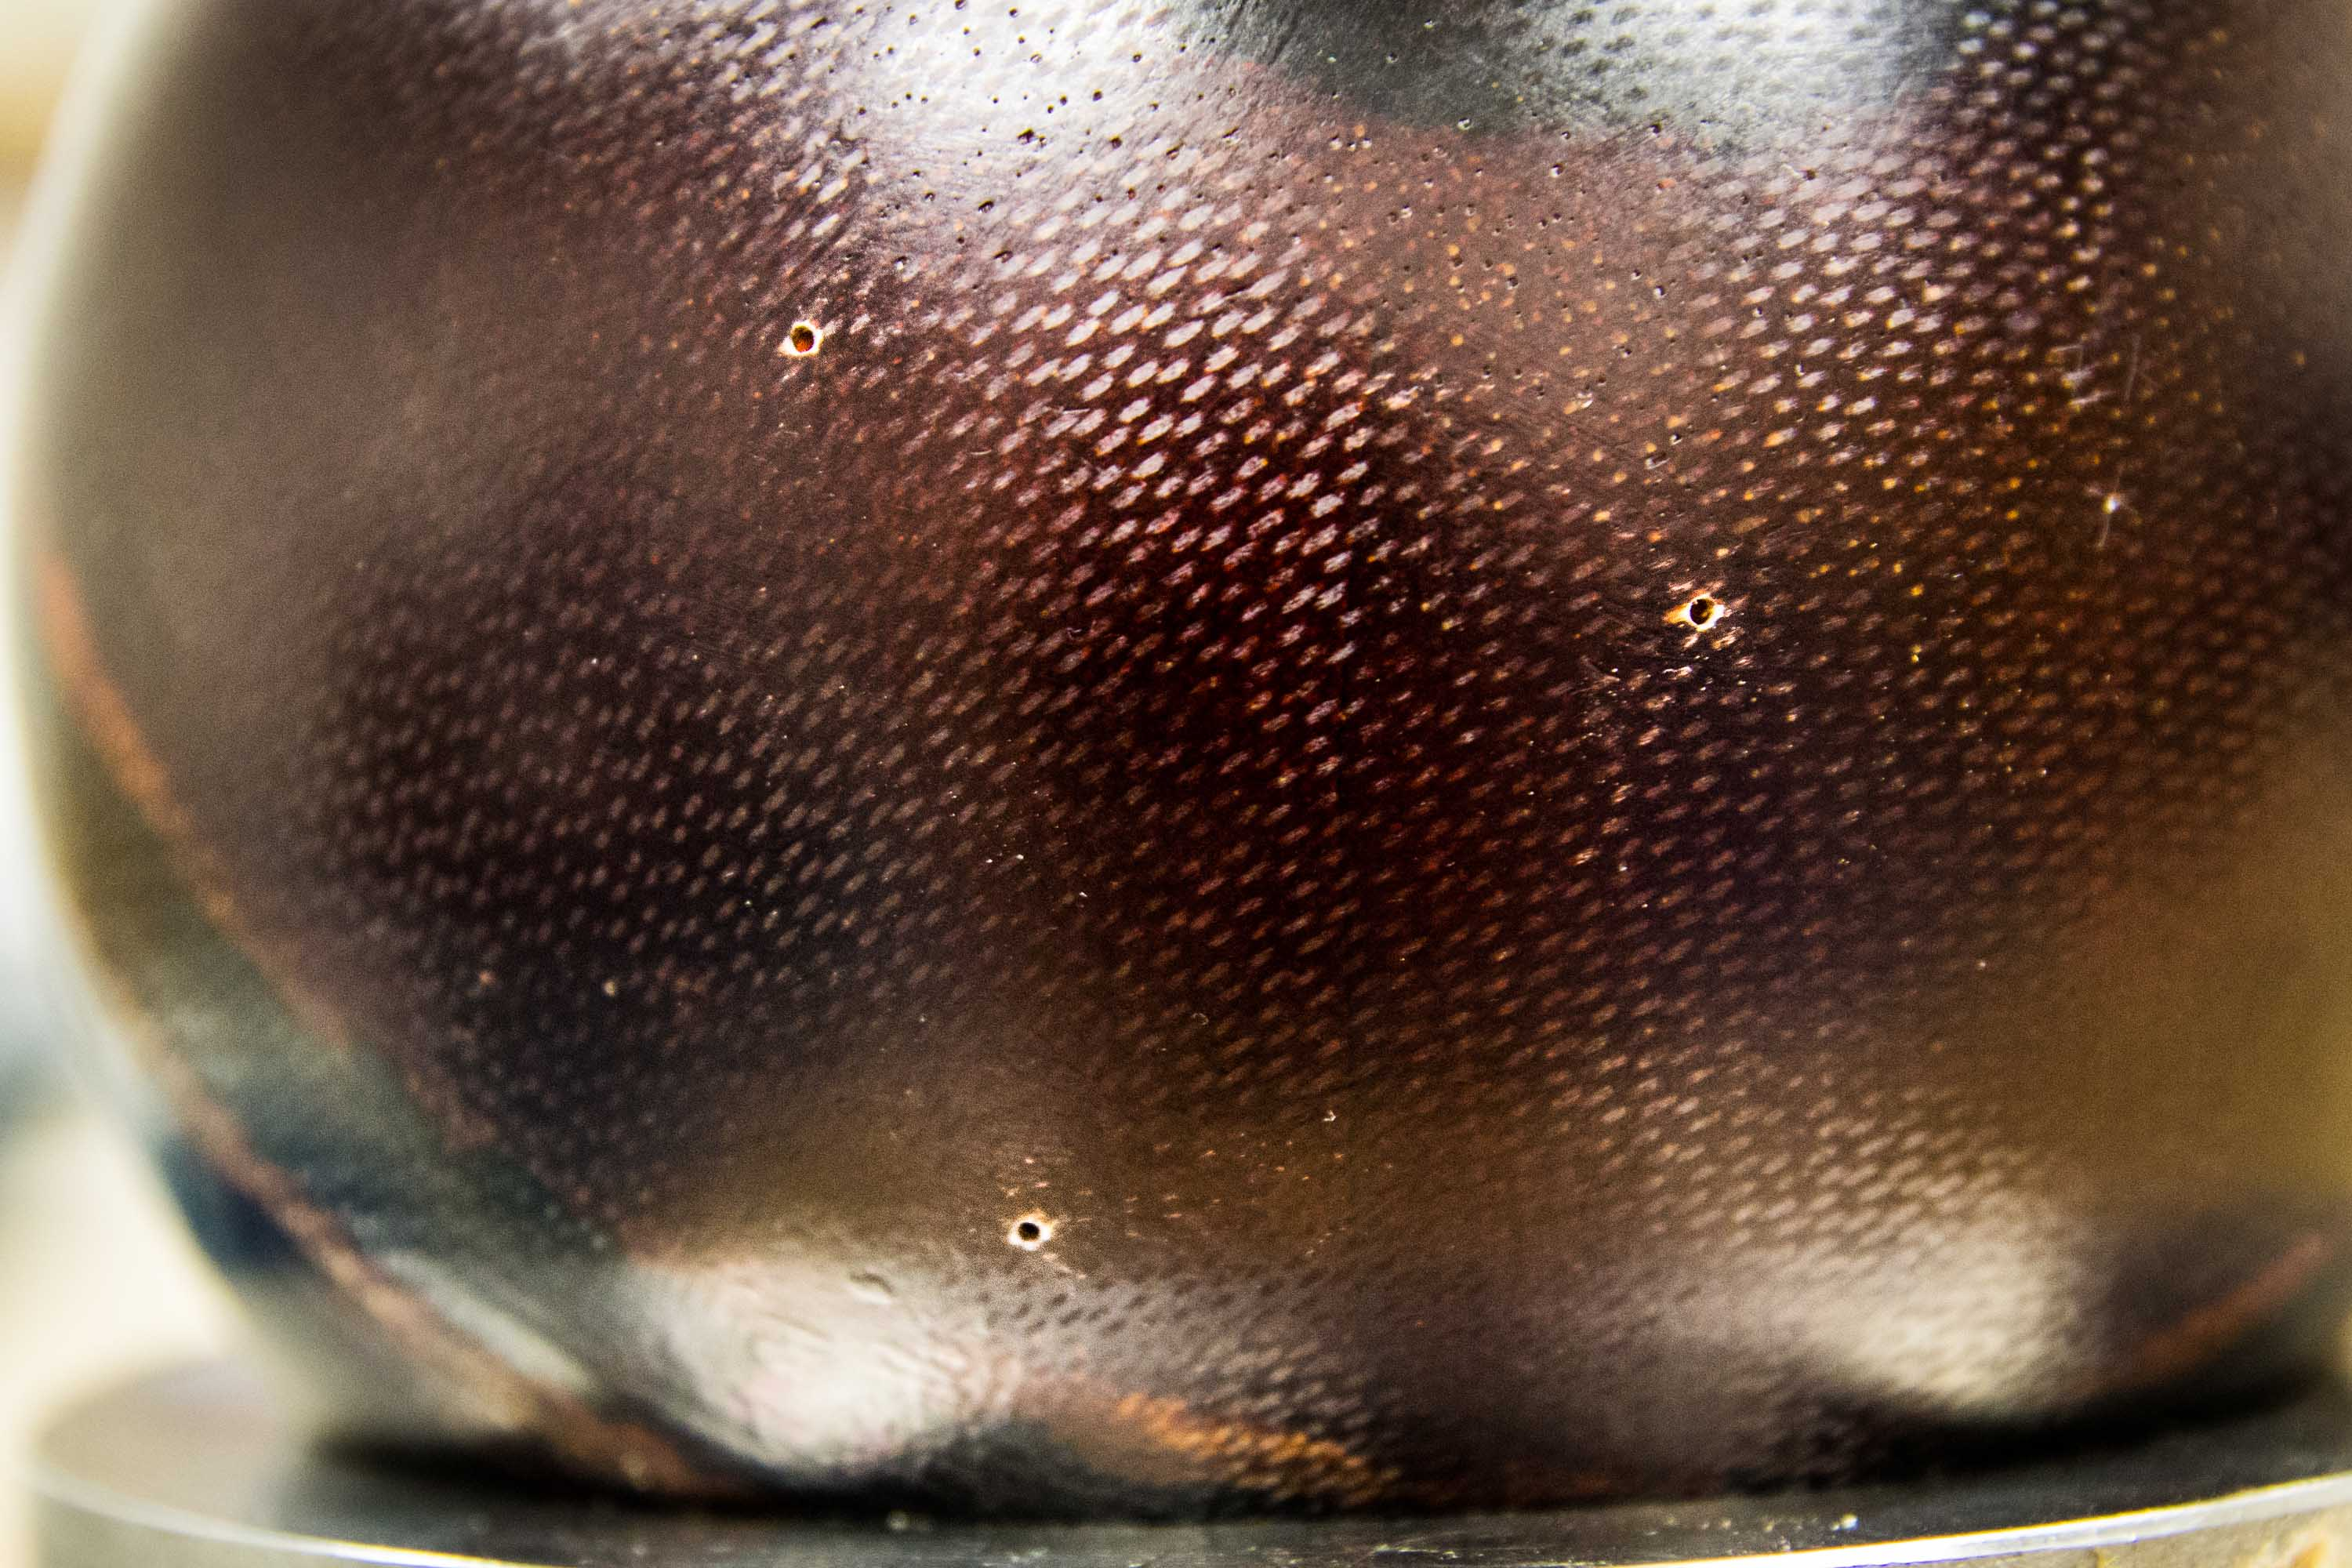
\includegraphics[clip=true,trim=0 0 0 126px]{Holes}
		\subcaption{}
	\end{subfigure}

	\caption{Small pins attached to the plastic ring (a), that fit into the 3 holes on the unit surface (b) make easy to mount the unit in the 6 different orientations.}
	\label{fig:PinsHoles}
\end{figure}

Once the unit can be mounted in the needed orientation, a total of 15 measurement series have to be performed. Eight are required to obtain the 3D center of gravity, one for the platform inertia and the additional six for the moment of inertia coefficients.
This is a very tedious process, and thus could be improved in the future.

As introduced before, we test each measurement series against the prediction, which is
\begin{align*}
	g_{\textup{t}} & =	\frac{mr}{s} \\
	I_{\textup{t}} & = mr^2
\end{align*}

as given in equations \eqref{eq:It} and \eqref{eq:gt}. The mean difference $\delta g$ is added, to place the two curves upon each other.
A nut of mass 10.55 g was used as a test mass for all series.
The results are given in figure \ref{fig:FFU} for the center of gravity measurements and the inertia tensor measurements.
No major deviations from the predicion could be observed.
Table \ref{tab:FFUCoG} lists the results from the center of gravity measurements.
Note, that the value $g_i - g_i'$ is abbreviated simply as $g_i$.
As one can see, the center of gravity is slightly displaced from the geometrical center of the unit by a about 4 millimeters with a relative deviation of about 5 \%.
However, as seen in the 2D center of gravity measurement in section \ref{sec:2DCoG}, there might be some systematic error, so the real center could be shifted by another few millimeters.

The results on the inertia measurements for the single axis are listed in table \ref{tab:FFUI}. Also listed there are the values for the parallel axis correction. Comparing these to the actual moments of inertia, their magnitude is very small, since the center of gravity lies close to the geometrical center.
The final result of the inertia tensor is given in table \ref{tab:FFUInertiaTensor}. The off-diagonal elements are very small, their values are even below the measured deviation.
Thus, we can conclude, that the unit is balanced in its geometrical frame.

\begin{table}
	\centering
	\begin{tabular}{r | r r}
		\multicolumn{3}{r}{rel. $\sigma$} \\
		& \multicolumn{2}{r}{2D center of gravity ($x-$ orientation)} \\
		\hline
		$g_{1}$	& 2.932(50) g	& 1.69 \% \\
		$g_{3}$	& 0.884(22) g	& 2.54 \% \\
		$R_x$	& -1.409(54) mm	& 3.87 \% \\
		$R_y$	& -6.15(10) mm	& 1.69 \% \\
		& \multicolumn{2}{r}{2D center of gravity ($z+$ orientation)} \\
		\hline
		$g_2$	& 0.730(37) g	& 5.05 \% \\
		$g_3$	& -0.84(10) g	& 12.46 \% \\
		$R_x$	& -2.92(29) mm	& 9.86 \% \\
		$R_y$	& -1.531(77) mm	& 5.05 \% \\
		& \multicolumn{2}{r}{3D center of gravity} \\
		\hline
		$R_x$	& -2.92(29) mm	& 9.86 \% \\
		$R_y$	& 2.309(75) mm	& 3.24 \% \\
		$R_z$	& -1.409(54) mm	& 3.87 \% \\
		& \multicolumn{2}{r}{Distance from origin} \\
		\hline
		$D$	& 3.73(17) mm	& 4.67 \% \\
	\end{tabular}
	\caption{Complete set of results for determining the 3D center of gravity of the \emph{MUSCAT FFU}. [\texttt{InertiaTensor.py}]}
	\label{tab:FFUCoG}
\end{table}

\begin{table}
	\centering
	\begin{tabular}{l | l l l l}
		axis	& I [$\unit{g\,m^2}$]		& rel. $\sigma$ & $R$ [mm]		& $m R^2$ [$\unit{g\,m^2}$] \\
		\hline
		$xx$	& 2.283(89) & 3.91 \%	& 2.70	& 0.0030 \\
		$yy$	& 2.189(73) & 3.32 \% 	& 3.24	& 0.0043 \\
		$zz$	& 2.404(97) & 4.02 \% 	& 3.72	& 0.0057 \\
		$xy$	& 2.25(15) & 6.80 \% 	& 3.96	& 0.0065 \\
		$xz$	& 2.384(79) & 3.31 \%	& 2.54	& 0.0027 \\
		$yz$	& 2.43(20) & 8.30 \%	& 3.93	& 0.0064 \\
	\end{tabular}
	\caption{Moment of inertia measurements of the \emph{MUSCAT FFU} along the axes to compute the inertia tensor. Also given is the perpendicular distance of each axis to the 3D center of gravity, as well as the resulting correction $mR^2$ from the parallel axis theorem. [\texttt{InertiaTensor.py}]}
	\label{tab:FFUI}
\end{table}

\begin{table}
	\centering
	\begin{tabular}{l | r r}
		axis	& I [$\unit{g\,m^2}$]		& rel. $\sigma$ \\
		\hline
		$I_p$		& 244.9(15)	& 0.61 \% \\
		$I_{xx}$	&	2.283(89)	& 3.91 \% \\
		$I_{yy}$	&	2.189(73)	& 3.32 \% \\
		$I_{zz}$	&	2.404(97)	& 4.02 \% \\
		$I_{xy}$	&	0.02(13)	& - \\
		$I_{xz}$	&	0.04(14)	& - \\
		$I_{yz}$	&	0.14(23)	& - \\
	\end{tabular}
	\caption{The inertia tensor of the \emph{MUSCAT FFU}. [\texttt{InertiaTensor.py}]}
	\label{tab:FFUInertiaTensor}
\end{table}

\section{Implementation}

The code to analyze the measurement results is written in \emph{Python} and relies heavily on \emph{numpy}, \emph{scipy} and \emph{matplotlib}.
Experimental data is read from \emph{JSON} (JavaScript Object Notation) files.
The complete project is available in the repository on \emph{GitHub} at \cite{website:github}.
And includes all script, which were used to create the plots in this report.
Thus, all the measurements results are also stored in the repository. 

The video tracker tool is written in \emph{C++} and thus has to be compiled for the platform in use. The code is mostly adapted from the website \cite{website:opencv}.

It was tried to keep the code as modular as possible and to reuse existing code. Thus, the actual scripts to perform the calculations in the report mostly consist of reading in the data from the \emph{JSON} files and calling a function to analyze the measurement series.
Each section, which contains analysis of measurement results is carried out by another script in the main folder of the repository. The script names, which were used to obtain the values and plots are given for reference on each table and figure shown in this report.
Each script outputs the measurement values on the console and writes the diagrams into the \texttt{out} folder 


% An example of a floating figure using the graphicx package.
% Note that \label must occur AFTER (or within) \caption.
% For figures, \caption should occur after the \includegraphics.
% Note that IEEEtran v1.7 and later has special internal code that
% is designed to preserve the operation of \label within \caption
% even when the captionsoff option is in effect. However, because
% of issues like this, it may be the safest practice to put all your
% \label just after \caption rather than within \caption{}.
%
% Reminder: the "draftcls" or "draftclsnofoot", not "draft", class
% option should be used if it is desired that the figures are to be
% displayed while in draft mode.
%
%\begin{figure}[!t]
%\centering
%\includegraphics[width=2.5in]{myfigure}
% where an .eps filename suffix will be assumed under latex, 
% and a .pdf suffix will be assumed for pdflatex; or what has been declared
% via \DeclareGraphicsExtensions.
%\caption{Simulation Results.}
%\label{fig_sim}
%\end{figure}

% Note that IEEE typically puts floats only at the top, even when this
% results in a large percentage of a column being occupied by floats.


% An example of a double column floating figure using two subfigures.
% (The subfig.sty package must be loaded for this to work.)
% The subfigure \label commands are set within each subfloat command,
% and the \label for the overall figure must come after \caption.
% \hfil is used as a separator to get equal spacing.
% Watch out that the combined width of all the subfigures on a 
% line do not exceed the text width or a line break will occur.
%
%\begin{figure*}[!t]
%\centering
%\subfloat[Case I]{\includegraphics[width=2.5in]{box}%
%\label{fig_first_case}}
%\hfil
%\subfloat[Case II]{\includegraphics[width=2.5in]{box}%
%\label{fig_second_case}}
%\caption{Simulation results.}
%\label{fig_sim}
%\end{figure*}
%
% Note that often IEEE papers with subfigures do not employ subfigure
% captions (using the optional argument to \subfloat[]), but instead will
% reference/describe all of them (a), (b), etc., within the main caption.


% An example of a floating table. Note that, for IEEE style tables, the 
% \caption command should come BEFORE the table. Table text will default to
% \footnotesize as IEEE normally uses this smaller font for tables.
% The \label must come after \caption as always.
%
%\begin{table}[!t]
%% increase table row spacing, adjust to taste
%\renewcommand{\arraystretch}{1.3}
% if using array.sty, it might be a good idea to tweak the value of
% \extrarowheight as needed to properly center the text within the cells
%\caption{An Example of a Table}
%\label{table_example}
%\centering
%% Some packages, such as MDW tools, offer better commands for making tables
%% than the plain LaTeX2e tabular which is used here.
%\begin{tabular}{|c||c|}
%\hline
%One & Two\\
%\hline
%Three & Four\\
%\hline
%\end{tabular}
%\end{table}


% Note that IEEE does not put floats in the very first column - or typically
% anywhere on the first page for that matter. Also, in-text middle ("here")
% positioning is not used. Most IEEE journals use top floats exclusively.
% Note that, LaTeX2e, unlike IEEE journals, places footnotes above bottom
% floats. This can be corrected via the \fnbelowfloat command of the
% stfloats package.

\section{Conclusion}

We have developed a method for testing the basic functions of the measurement like measuring the shift of the center of gravity caused by placing an object onto the platform as well as the moment of inertia of the whole system.
These have then been combined to measure the center of gravity of the object first in two dimensions, then finally in 3 dimensions.
This information helped us to correct the measured moment of inertia coefficients, which where then used to compute the complete inertia tensor.

While there was some deviation between the measured center of gravity in two dimensions and the predicted position, the measurements themselves show only small relative standard deviations in the order of 1 \% in the experiments.
However, the difference between the experimental value and the prediction has to be investigated more thoroughly in a future work.

The moment of inertia measurement of the platform has been done with a quite high precision, giving only a relative standard deviation of 0.1 \%.
But since the platform moment is much higher than the that of the actual unit being measured, this precision may not be sufficient for many cases.
As can be seen, the relative standard deviation on the \emph{MUSCAT FFU} measurements goes up to 8.3 \%!
This precision could maybe easily be increased by just capturing longer videos with the \emph{GoPro} camera.
Another way to increase the precision might be the use of the general expression of eq. \ref{eq:I} as found in \cite{report:ernest}.

Finally, all the code is given to combine the measurements to a complete determination of the inertia tensor. Nevertheless, an error analysis of this computation has yet to be done, in order to identify the inputs, that are most crucial in the precision of the single coefficients. This could also be part of some future work.

% if have a single appendix:
%\appendix[Proof of the Zonklar Equations]
% or
%\appendix  % for no appendix heading
% do not use \section anymore after \appendix, only \section*
% is possibly needed

% use appendices with more than one appendix
% then use \section to start each appendix
% you must declare a \section before using any
% \subsection or using \label (\appendices by itself
% starts a section numbered zero.)
%



% Can use something like this to put references on a page
% by themselves when using endfloat and the captionsoff option.
\ifCLASSOPTIONcaptionsoff
  \newpage
\fi



% trigger a \newpage just before the given reference
% number - used to balance the columns on the last page
% adjust value as needed - may need to be readjusted if
% the document is modified later
%\IEEEtriggeratref{8}
% The "triggered" command can be changed if desired:
%\IEEEtriggercmd{\enlargethispage{-5in}}

% references section

% can use a bibliography generated by BibTeX as a .bbl file
% BibTeX documentation can be easily obtained at:
% http://www.ctan.org/tex-archive/biblio/bibtex/contrib/doc/
% The IEEEtran BibTeX style support page is at:
% http://www.michaelshell.org/tex/ieeetran/bibtex/
%\bibliographystyle{IEEEtran}
% argument is your BibTeX string definitions and bibliography database(s)
%\bibliography{IEEEabrv,../bib/paper}
%
% <OR> manually copy in the resultant .bbl file
% set second argument of \begin to the number of references
% (used to reserve space for the reference number labels box)
\begin{thebibliography}{1}

\bibitem{book:goldstein}
H.~Goldstein, C.~Pool, J.~Safko, \emph{Classical Mechanics}, 3rd Ed. June 25, 2001

\bibitem{report:ernest}
Ernest~Company~Vallet, \emph{A method for determining and balancing the mass properties of
the Free Flying Units}, February 11, 2014

\bibitem{website:opencv}
\url{http://www.aishack.in/2010/07/tracking-colored-objects-in-opencv/}

\section*{Source code repository}
\bibitem{website:github}
\url{https://github.com/morloy/trifilar-mass-prop}

\end{thebibliography}

% biography section
% 
% If you have an EPS/PDF photo (graphicx package needed) extra braces are
% needed around the contents of the optional argument to biography to prevent
% the LaTeX parser from getting confused when it sees the complicated
% \includegraphics command within an optional argument. (You could create
% your own custom macro containing the \includegraphics command to make things
% simpler here.)
%\begin{IEEEbiography}[{\includegraphics[width=1in,height=1.25in,clip,keepaspectratio]{mshell}}]{Michael Shell}
% or if you just want to reserve a space for a photo:
% insert where needed to balance the two columns on the last page with
% biographies
%\newpage


% You can push biographies down or up by placing
% a \vfill before or after them. The appropriate
% use of \vfill depends on what kind of text is
% on the last page and whether or not the columns
% are being equalized.

%\vfill

% Can be used to pull up biographies so that the bottom of the last one
% is flush with the other column.
%\enlargethispage{-5in}

\clearpage
\appendices

\section{Instructions on determining the inertia tensor}
\label{sec:Instructions}

In this section, we describe the necessary steps to do a full measurement of the inertia tensor.

\paragraph{Preparations}
\begin{itemize}
	\item Choose a test weight, e.~g. a small nut.
	\item Choose the positions to place the nut on a arm for the measurement series, e.~g. 30--70 cm in steps of 10 cm.
	\item Make sure, that you can mount the unit in all required orientations $xx, yy, zz, xy, xz, yz$, with the center of these axes vertically aligned at the platform center. 
\end{itemize}

\paragraph{Center of gravity}
\begin{enumerate}
	\item Choose two orientations on the main axes, e.~g. $xx$ and $zz$.
	\item For each orientation, perform the measurement of the 2D center of gravity:
		\begin{enumerate}
			\item Place the unit at the platform in the given orientation.
			\item Raise the central spike and the two support points with the scales.
			\item Use a bubble level on each supported arm to align the platform to the $xy$ plane.
			\item For each supported arm, take a measurement series.
				\begin{enumerate}
					\item For each position, place the test mass and note the value on the scale.
				\end{enumerate}
			\item Remove the unit.
			\item Take a measurements series again on each arm, that has been supported when the unit was placed on the platform. The test mass makes the arm stay on the support point.
		\end{enumerate}
\end{enumerate}

\paragraph{Inertia tensor}

\begin{enumerate}
	\item Lower the central spike and the support point, such that the platform can move freely again.
	\item Point the laser on the mirror on arm 3, such that it is visible on the paper sheet at the wall.
	\item Switch off the room lighting and use the desk lamp instead. The laser dot then becomes clearly visible.
	\item For each orientation, place the unit on the platform and perform a measurement series.
		\begin{enumerate}
			\item Place the test mass at the desired position.
			\item Rotate the platform by a small degree, such that the laser dot on the wall moves by about 10 cm.
			\item Record a video with the \emph{GoPro} camera of at least 7 seconds. For this purpose, the WiFi remote is very useful.
		\end{enumerate}
	\item Remove the unit and perform one measurement series with the platform alone.
	\item Copy the video files from the $GoPro$ camera and rename them after the scheme \texttt{axis/position.MP4}. The position of the test mass must given in meters with two decimals, e.~g. \texttt{xx/0.30.MP4}. This means, that there is a seperate folder for each orientation.
\end{enumerate}

\paragraph{Use the code}

To apply the code on the just taken measurements, the results must be entered in a \emph{JSON} file. As a starting point, the file \emph{FFU.json} should be used, which is also attached to this document for reference.
Now follows a short description of the parameters found in the file.

\begin{enumerate}
	\item Masses are given in \emph{kg} for parameters \texttt{unit mass, platform mass} and \texttt{test mass}.
	\item \texttt{positions} are given in \emph{m}.
	\item Center of gravity measurements in \texttt{cog}
		\begin{enumerate}
			\item \texttt{axes} describes the two axes in which the 2D CoGs were measured. Currently supported are ``xy'', ``xz'' and ``yz''. The later measurement series must be given in exactly this order!
			\item \texttt{data} holds two measurement series, one for each CoG in the order given in \texttt{axes}.
				\begin{enumerate}
					\item \texttt{name} can be freely chosen and is displayed in the output to make the result more readable.
					\item \texttt{free arm} gives the arm, that is not supported by a support point.
					\item \texttt{series} contains the measurement series for $g_i$ and $g_i'$.
						\begin{enumerate}
							\item \texttt{name} another freely chosable name.
							\item \texttt{data} series for $g_i$ in \emph{gram}!
							\item \texttt{platform} series for $g_i'$ in \emph{gram}!
						\end{enumerate}
				\end{enumerate}
		\end{enumerate}
	\item \texttt{initial parameters} have to be given for the least-square fit performed on the filmed inertia wave. These parameters are critical for the success of the fit. If the fit fails, a list of the previously successful parameters is printed. These can be copied into the \emph{JSON} file for the next try. They are given in the order $A_1, \tau_1, T_1, \delta_1, A_2, \tau_2, T_2, \delta_2, C$, as they appear in eq. \eqref{eq:FitFunction}.
\end{enumerate}

When the file is prepared, it has to be stored in the same directory, which holds also the video files from the inertia measurements.

Finally, the script \texttt{InertiaTensor.py} can be used. The name and path to the \emph{JSON} file is given in the script itself, and thus has to be adjusted.
If the script runs without errors, it should output a list of all variable as they appear in tables \ref{tab:FFUCoG}, \ref{tab:FFUI} and \ref{tab:FFUInertiaTensor}.


\clearpage
\section{Constructing axes on a sphere}
\label{seq:ConstructAxes}

The outer appearance of the \emph{MUSCAT FFU} consists of two hemispheres and a hole for an electrical connector. The sphere has a radius of $r =$ 6.2 mm.
Since we need to mount it in 6 different orientations on the platform, there was a need to construct the main axes on the surface, which have a right angle between each other, as well as the diagonal axes, which are inclined at 45 degrees relative to the main axes.
Additionaly, these axes have to be aligned to the reference frame of the platform.

The construction was finally carried out using a compass and some geometrical considerations to construct a circle with an arbitrary perpendicular radius on the sphere surface.
For this reason, a formula was derived to calculate the radius of compass circle needed to draw a circle of radius $R$ on the surface of the sphere.
Looking at figure \ref{fig:CircleConstruction}, we want to find the length $c$ in dependence of the radius $r$ of the sphere and the radius $R$ of the circle, we want to construct.

The fomula then can be found as
\begin{align}
	a & = \sqrt{r^2 - R^2} \\
	b & = r - a \\
	c(R) & \equiv \sqrt{R^2 + b^2}\\
	& = \sqrt{2r^2 - 2r \sqrt{r^2 - R^2}} \\
	& = r \sqrt{2 \left(  1 - \sqrt{1 - \left( \frac{R}{r} \right)^2 } \right)}
	\label{eq:cR}
\end{align}

Now, by using this formula for $R = r$, we can draw the equator for a given point on the sphere.
In this case the equation eq. \eqref{eq:cR} reduces to
\begin{align}
	c(R=r) & = \sqrt{2}~r
\end{align}

Taking an arbitrary point and drawing the equator and then drawing the next equator from another point on the equator line, we can construct the main axes, which have an angle of 90 degree to each other.

The next step is to draw the diagonal axes. For this purpose, we use $R = r \sin \frac{\pi}{4} = \frac{r}{\sqrt{2}}$ and thus find
\begin{align}
	c\left(R = \frac{r}{\sqrt{2}} \right) & = \sqrt{2 - \sqrt{2}}~r
\end{align}

By drawing circles of this radius around each axis point, we find the diagonal axes at the circle intersections.

Finally, we want to mark the circle, where the plastic disk touches the surface, when the unit is placed on the platform.
The plastic disk has an inner radius of $R = $ 9.14 mm. To draw this ring on the sphere, we thus need to set the compass to $c \approx$ 5 mm.

When drawing these circles around each of the 6 axis points, it has been observed, that they intersect at exaclty 3 points, where each circle has 2 intersection points.
This was then the reason to drill tiny holes into the sphere surface and attach pins to the plastic ring.
With this setup, the unit can now be mechanically fixed to the platform in one of the 6 orientations.

\begin{figure}
	\centering
	\definecolor{qqwuqq}{rgb}{0,0.39,0}
	\begin{tikzpicture}[line cap=round,line join=round,>=triangle 45,x=0.8cm,y=0.8cm]
	\draw [shift={(0,0)},color=qqwuqq,fill=qqwuqq,fill opacity=0.1] (0,0) -- (0:1.39) arc (0:53.13:1.39) -- cycle;
	\draw (0,0)-- (3,4);
	\draw [line width=1.2pt] (3,4)-- (3,-4);
	\draw [line width=1.2pt,dash pattern=on 3pt off 3pt] (3,4)-- (5,0);
	\draw (0,0)-- (3,0);
	\draw (3,0)-- (5,0);
	\draw (0,5)  arc(90:-90:5);
	\begin{scriptsize}
	\draw[color=black] (1.38,2.4) node {$r$};
	\draw[color=qqwuqq] (1.08,0.41) node {$\theta$};
	\draw[color=black] (2.56,0.74) node {$R$};
	\draw[color=black] (3.72,2.01) node {$c$};
	\draw[color=black] (1.59,-0.19) node {$a$};
	\draw[color=black] (4.09,-0.19) node {$b$};
	\end{scriptsize}
	\end{tikzpicture}
	\caption{Cross-section of a sphere with radius $r$. Here $R$ denotes the perpendicular radius of a circle on the surface and $c$ gives the distance to be used on the compass to construct the given circle.}
	\label{fig:CircleConstruction}
\end{figure}

\onecolumn

\section{Inertia tensor measurements curves}

\begin{figure}[h]
	\centering
	\setkeys{Gin}{width=0.30\linewidth}
	\includegraphics{InertiaTensor/gx1}
	\includegraphics{InertiaTensor/gx1p}
	\includegraphics{InertiaTensor/gx3}
	\includegraphics{InertiaTensor/gx3p}
	\includegraphics{InertiaTensor/gz2}
	\includegraphics{InertiaTensor/gz2p}
	\includegraphics{InertiaTensor/gz3}
	\includegraphics{InertiaTensor/gz3p}
	\includegraphics{InertiaTensor/platform}
	\includegraphics{InertiaTensor/xx}
	\includegraphics{InertiaTensor/yy}
	\includegraphics{InertiaTensor/zz}
	\includegraphics{InertiaTensor/xy}
	\includegraphics{InertiaTensor/xz}
	\includegraphics{InertiaTensor/yz}
	\caption{Complete set of measurement curves for the inertia tensor of the \emph{MUSCAT FFU}. Shifted upon theoretical predictions $g_{\textup{t}}$ and $I_{\textup{t}}$ to verify the linear/quadratic shape. [\texttt{InertiaTensor.py}]}
	\label{fig:FFU}
\end{figure}


\clearpage

\section{Sample data}

\includecode{FFU.json}

% that's all folks
\end{document}
